% Template for a Computer Science Tripos Part II project dissertation
\documentclass[12pt,a4paper,twoside,openright]{report}
\usepackage[pdfborder={0 0 0}]{hyperref}    % turns references into hyperlinks
\usepackage[margin=25mm]{geometry}  % adjusts page layout
\usepackage{graphicx, color}  % allows inclusion of PDF, PNG and JPG images
\usepackage{verbatim}
\usepackage{docmute}   % only needed to allow inclusion of proposal.tex
\usepackage{dsfont, amsmath, textcomp}
\usepackage{pdfpages}
\usepackage{listings}
\usepackage{booktabs}
\usepackage[table,xcdraw]{xcolor}
\definecolor{mygray}{rgb}{0.8,0.8,0.8}
\usepackage{caption,inconsolata}
\DeclareCaptionFont{black}{\color{black}}
\DeclareCaptionFormat{listing}{%
  \parbox{\textwidth}{\colorbox{white}{\parbox{\textwidth}{#1#2#3}}\vskip-4pt}}
\captionsetup[lstlisting]{format=listing,labelfont=black,textfont=black}
\lstset{frame=tlrb,xleftmargin=\fboxsep,xrightmargin=-\fboxsep,basicstyle=\ttfamily \footnotesize,breaklines=true}
\usepackage{multicol}
\usepackage{multirow}
\usepackage[symbol]{footmisc}
\usepackage{float}
\usepackage{forest}
% \usepackage{titlesec}
\usepackage[T1]{fontenc}
\usepackage{wrapfig}
\usepackage[all]{nowidow}
\usepackage{newtxtext,newtxmath}
% \usepackage[lmr]{lmodern}
% \usepackage{newpxtext,newpxmath}
% \usepackage[garamond]{mathdesign}
% \usepackage{biblatex}
\usepackage{bigfoot}


\raggedbottom                           % try to avoid widows and orphans
\sloppy
\clubpenalty1000%
\widowpenalty1000%

% \usepackage[utf8]{inputenc}
\usepackage[UKenglish]{babel}
\usepackage[UKenglish]{isodate}
% \usepackage[backend=biber, style=numeric]{biblatex}
% \addbibresource{refs.bib}

\renewcommand{\baselinestretch}{1.1}    % adjust line spacing to make

%###########################################################################
\newcommand{\projectTitle}{\bf Investigating the effect of \\
 & \bf Translation Quality on Summarisation Quality}
 \newcommand{\name}{Anish Das}
 % more readable

 \newcommand{\red}[1]{\textcolor{red}{#1}}
 \newcommand{\todo}[1]{\red{\textbf{TODO}: #1}}
 \newcommand{\query}[1]{\red{\textbf{Query}: #1}}

 \newcommand{\bleu}{\textsc{Bleu} }
 \newcommand{\rouge}{\textsc{Rouge} }
 \newcommand{\perftrans}{\textsc{Perf-Trans} }


 \newcommand{\changedFont}[1]{{\fontfamily{qcr}\selectfont #1}}
 \newcommand{\fone}{$F_1$}

 \newenvironment{specialfootnote}
    {
    \renewcommand*{\thefootnote}{\fnsymbol{footnote}}
    }
    {
    \renewcommand*{\thefootnote}{\arabic{footnote}}
    }

\newcommand{\quickwordcount}{%
  \immediate\write18{texcount -1 -sum -merge -q main.tex > main-words.sum }%
  \input{main-words.sum} words%
}


 %###############################################################

\begin{document}
 \renewcommand*{\thefootnote}{\arabic{footnote}}

\bibliographystyle{plain}


%%%%%%%%%%%%%%%%%%%%%%%%%%%%%%%%%%%%%%%%%%%%%%%%%%%%%%%%%%%%%%%%%%%%%%%%
% Title

%TC:ignore
\pagestyle{empty}

\rightline{\LARGE \textbf{\name}}

\thispagestyle{empty}
\vspace*{60mm}
\begin{center}
\Huge
\textbf{Investigating the effect of \\Translation Quality on \\Summarisation Quality}\\[5mm]
Computer Science Tripos -- Part II\\[5mm]
Trinity Hall \\[5mm]
\includegraphics[width=0.2\textwidth]{figs/TrinityHall.pdf}\\

\today  % today's date
\end{center}

\pagenumbering{roman}


%%%%%%%%%%%%%%%%%%%%%%%%%%%%%%%%%%%%%%%%%%%%%%%%%%%%%%%%%%%%%%%%%%%%%%%%%%%%%%
% Proforma, table of contents and list of figures
% \cleardoublepage
\pagestyle{plain}

\newpage
% \phantom{.}
% \thispagestyle{empty}
% \newpage
\setcounter{page}{1}
\section*{Declaration}

I, Anish Das of Trinity Hall, being a candidate for Part II of the Computer Science Tripos, hereby declare
that this dissertation and the work described in it are my own work,
unaided except as may be specified below, and that the dissertation
does not contain material that has already been used to any substantial
extent for a comparable purpose.
I am content for my dissertation to be made available to the students and staff of the University.

\bigskip
\leftline{Signed: Anish Das}

\medskip
\leftline{Date [date]}

\chapter*{Proforma}

{\large
\begin{tabular}{ll}
Name:               & \bf 2333C                      \\
College:            & \bf Trinity Hall                     \\
Project Title:      &  \projectTitle \\
Examination:        & \bf Computer Science Tripos -- Part II, June 2021  \\
Word Count:         & \bf \quickwordcount \footnotemark[1]\\
Lines of Code:      & \bf 1585\footnotemark[2]  \\
Project Originator: & Dr Andrew Caines \& Dissertation Author                \\
Supervisor:         & Dr Andrew Caines \& Dr Zheng Yuan                   \\
\end{tabular}
}
\footnotetext[1]{Calculated using:
\texttt{\detokenize{\immediate\write{texcount -1 -merge -q main.tex > main-words.sum}}} and
\texttt{\detokenize{\input{main-words.sum} words}}\\
(\lstinline{\%TC:ignore ... \%TC:endigore}) was applied around the content before Introduction and after Conclusion.}
%the Proforma Chapter and the contents following the Conclusion}
\footnotetext[2]{Calculated using: \lstinline{git ls-files | grep `\\.py' | xargs wc -l}. This doesn't include the `.ipynb' (colab notebooks) but that was minimal.}

\stepcounter{footnote}


\section*{Original Aims of the Project}
This project seeks to investigate the effect of translation quality on summarisation quality in order to estimate the feasibility of a Cross-Lingual Summarisation to be scaled in the absence of good translation models. It involved training Neural Machine Translation (NMT) models using the Transformer architecture for multiple source languages into English. The next was applying a pre-trained state-of-the-art summarisation model to the translations produced by the models. The final step involved testing the correlation between the \bleu scores (translation metric) and the \rouge scores (summarisation metric).

\section*{Work Completed}
This project has been successful in achieving the success criteria listed in the project proposal.
First, the Transformer architecture was built from scratch and used to create multiple translation models by saving the parameters at regular intervals during the training process. The checkpointed translation models have been used to translate the documents in the evaluation GV-crowd/snippet dataset from\cite{nguyen-daume-iii-2019-global}. The translated sentences were then summarised. The \bleu and \rouge metrics were calculated along with a quantitative comparison of the two scores.

\newpage
\section*{Special Difficulties}
No special difficulties were encountered, apart from having to adjust to the COVID-19 pandemic.


% \red{Learning how to training Transformers is a difficult task that requires proper care towards various factors.
% And having to work remotely for the entire year.}

\section*{Acknowledgements}

A huge thanks to my supervisors, Andrew P. Caines and Zheng Yuan, whose support throughout the project was  immense. Further, I would like to extend my gratitude to my Director
%TC:endignore
 of Studies, Simon W. Moore, for his comments to help polish this dissertation.
\\
Thank you for reading.

\tableofcontents

\listoffigures
% \listoftables
% \lstlistoflistings



%%%%%%%%%%%%%%%%%%%%%%%%%%%%%%%%%%%%%%%%%%%%%%%%%%%%%%%%%%%%%%%%%%%%%%%
% now for the chapters

\pagestyle{headings}

\cleardoublepage\pagenumbering{arabic}

%%%%%%%%%%%%%%%%%%%%%%%%%%%%%%%%%%%%%%%%%%%%%%%%%%%%%%%%%%%%%%%%%%%%%%%%%%%%%%%%%%%%%%%%%%%%%%%%%%%%%
%%%%%%%%%%%%%%%%%%%%%%%%%%%%%%%%%%%%%%%%%%%%%%%%%%%%%%%%%%%%%%%%%%%%%%%%%%%%%%%%%%%%


\chapter{Introduction}
\label{intro}


% Natural Language Processing (NLP) is a branch of Artificial Intelligence (A.I.) that seeks to bridge the gap between human communication and computer understanding. It incorporates and draws from many disciplines, including computer science and computational linguistics.

\section{Motivation}
\label{motivation}

Within this vast and varied field of NLP lies the task of Cross-Lingual Summarisation (CLS), which aims to produce a summary in one specific target language from a source document in another languages. This is an essential task because it will lift the language barrier, for example enabling easy access to information for all. However, the amount of textual data on the internet is immense and continues to grow day by day. Today it is impossible to keep up with it because a person simply does not have enough time to read it all. By summarising the data, we trim it down to its most salient points, which can be consumed quickly, thus, allowing humans to consume a more significant amount of information and in a shorter amount of time.  Suppose a CLS system is deployed on a large scale: it will bring about an exponential increase in the amount of information available to everyone and thus empower humans with the knowledge of the diverse world we live in today. Such a system will have immense and varied applications, for example, providing news from all over the world (very important in countries where the news can be very biased), access to information for academic purposes (there are already annual conferences on medical paper translations which reflects their importance), access to public health information in global health emergencies and many more, all in a condensed format.

\section{Project Focus}
\label{project-focus}

CLS has two main steps: first, \textbf{translating} the source document into a target language and second, \textbf{summarising} the translated text. Since CLS is a two-step process, any errors in the first step will be carried forward and possibly amplified through the second step and end up in the resulting summary. Further, it is widely known that we require large sentence-aligned datasets to build good quality translation models now that machine translation is largely driven by neural networks. Language pairs that have these large datasets are called `high-resource' in the NLP community and those without are called `low-resource' language pairs. The general trend with NMT and corpus size is shown in the Figure \ref{fig:corpus-size-vs-bleu} from paper\cite{translation-six}. Particularly, note that the green-line representing NMT improves as the corpus size is increased. Therefore, translation models trained on `\textit{low-resource}' language pairs do not come across enough sentences and end up having quite a few inaccuracies in their translations. This raises the question of whether bad-quality translations will adversely affect the information content and the readability of the resultant summary.



\begin{figure}
    \centering
    \includegraphics[width=0.45\textwidth]{figs/corpus-size-vs-bleu.PNG}
    \caption{The variation of BLEU scores with respect to the corpus sizes. }
    \label{fig:corpus-size-vs-bleu}
\end{figure}

Since there are language pairs which are `\textit{low-resource}', it is necessary to ascertain the feasibility of building a CLS system for such language-pairs.
With this as a foundation, through this project, I want to explore the effect of translation quality on summarisation quality. To achieve this I will be creating, training, and comparing translation models of differing quality. Moreover, I will also be comparing the summaries produced against the baselines i.e. the hand-written summaries and web-scraped summaries. Translation models, like most machine learning systems, improve with more training and therefore, a model's features are check-pointed at regular intervals yielding models of varying quality. The earlier models will be used as proxy for worse translation models and the later models for better translation models.

\section{Related Work}
\label{related-work}
My project is inspired by the paper\cite{nguyen-daume-iii-2019-global}, the authors set out to build a dataset for evaluating cross-lingual summarisation methods. They used the Global Voices\footnote{\url{https://globalvoices.org/}} to collect news articles in 15 different languages. Moreover, they crowd-sourced human summarisation of the articles collected in English and web-scraped the \textit{`snippet'} summaries available on the website as a gold standard reference. Finally, they trained four translation models, two of which were trained on a large scale dataset and the other two using a much smaller dataset, thus, yielding models with different quality. Finally, they compared the summaries from the resultant translations with ``\textit{gold-standard}'' using \rouge scores.
\newpage
\subsubsection{Example summaries}
% \begin{figure}[H]
%     % \centering
%     % \justify
%     {\changedFont{\input{figs/related-work-snippet-example.txt}}}
%     \caption{Example \textit{`snippet'} summary}
%     \label{fig:snippet-example}
% \end{figure}
\textbf{Example Crowd Summary}
\begin{lstlisting}
``There was a conference in Casablanca this past weekend for DABA. DABA is an association that aims to mobilize Morocco for the 2007 elections. They do this by training people in their citizen journalism skills, so that more people can hear about their issues.''
\end{lstlisting}
\textbf{Example Snippet Summary}
\begin{lstlisting}
``Morocco author Jillian York addressed a youth conference, organised by DABA, in conjunction with the National Democratic Institute's Morocco branch. The three-day event, which aimed at reevaluating political involvement in Morocco in the run-up to the 2007 legislative elections, also focused on building the capacity of young opinion leaders in citizen journalism skills, with an online emphasis in order to increase dialogue about issues of concern to youth.''
\end{lstlisting}

% \begin{figure}[H]
%     % \centering
%     % \justify
%     {\changedFont{\input{figs/related-work-crowd-example.txt}}}
%     \caption{Example \textit{`crowd'} summary}
%     \label{fig:crowd-example}
% \end{figure}


This project differs from\cite{nguyen-daume-iii-2019-global} in the following ways. Instead of using multiple language-pairs with different dataset sizes, this project considers multiple models of the same language pair and trained on the same dataset and only varying the time it has been trained. This project extends the investigation carried out by the authors, to compare multiple models of the same language pair as opposed to across different language pairs with differing dataset size. This idea was born from the intuition that some articles may be less compressible to begin with. Further, it is hard to conclusively compare the \bleu score between different languages. Therefore, to truly evaluate the effects of translation on summarisation, I wish to reduce the number of confounding variables, and thus, check-point models during the training process after every epoch were used instead.

The architecture used to implement the translation models is the Transformer architecture\cite{transformers}. Details of its conception and implementation are detailed in the following chapters. Finally, transformers are a deep architecture which are over 200\textsc{mb} in size, which makes them very unstable in the training process and the investigation carried out by Popel \& Bojar in the article\cite{training-tips} helped guide the training process.

% \section{Organisation of this Document}
% \label{doc-org}
% As per the requirements for this dissertation, there are chapters dedicated to the Preparation, Implementation, Evaluation and finally, a chapter Concluding the project and dissertation.

% \textbf{Chapter \ref{preperation} \nameref{preperation} }describes the work undertaken before programming commenced and also aims to build the theoretical basis needed to understand this document. It begins with a description of the \nameref{starting-point} and moves on to explaining the terms used throughout. Further, it details the background knowledge acquired during Step 1 of the software engineering process (Understanding the Core requirements and Feasibility Study). Finally, the project management decisions are stated which includes  Functional \& Non-Functional Requirements; Datasets used for training \& evaluation; the tools used and the platform where the project was run.

% \textbf{Chapter \ref{implementation} \nameref{implementation}} details the crux of the project, i.e. is the implementation of the Translation system and evaluating the summaries produced. It begins with a description of the pre-processing steps utilised, followed by a fine-grained explanation of the \nameref{transformer-architecture}. Finally, it explains the Training algorithm, the evaluation pipeline \& the mandatory Repository Overview along with all the decisions big/small with references to external resources which helped inform the choices made.

% \textbf{Chapter \ref{evaluation} \nameref{evaluation}}
% % \red{TODO: finish right after evaluation chapter}
% begins by describing the evaluation metrics used. Then it moves onto reporting the results of the evaluation and discussing the results along with any trends that appear. Finally, it discusses the qualitative features of the Output generated during the experiments.



%%%%%%%%%%%%%%%%%%%%%%%%%%%%%%%%%%%%%%%%%%%%%%%%%%%%%%%%%%%%%%%%%%%%%%%%%%%%%%%%%%%%%%%%%%%%%%%%%%%%%
%%%%%%%%%%%%%%%%%%%%%%%%%%%%%%%%%%%%%%%%%%%%%%%%%%%%%%%%%%%%%%%%%%%%%%%%%%%%%%%%%%%%
\chapter{Preparation}
\label{preperation}

\section{Starting Point}
\label{starting-point}
This project uses pre-trained summarisation models from the paper\cite{summary}.
All code in this project, for the translation model architecture, training algorithm, pre-processing and post-processing and finally evaluation code, was developed from scratch using some well-known libraries which are listed in the \nameref{project-management} section.
%The translation model was built from scratch after understanding the description in the paper\cite{transformers}.
The main focus of this project is in building/training/deploying translation models.


% \section{Relevant Terms}
% This section contains the definitions for many of the important terms used throughout this document to improve readability.

% \red{please let me know if I should add/remove any more terms here? Also Chapter one is wasting a ton of space. would it be okay to move this section there?}

% \begin{description}
%     \item[Sequence] A list of subwords or words is a Sequence. It can be a sentence in String format or a list of indices.
%     \item[Token-size] The number of tokens that are passed to the transformer in one training step. It is the product of the number of sequences and the length of each sequence in the batch.
%     \item[Throughput] The number of tokens digested by the transformer model in a second (typically used to refer to the training-throughput).
%     \item[Gold Standard] This is any text that is used in an NLP experiment which is hand-written and therefore is fluent with minimal grammatical errors.
% \end{description}



\section{Background Knowledge}
\label{background}
This section is meant to elaborate on content that is beyond the Part 1B in the Computer Science Tripos.
%and set the scene for the following Implementation and Evaluation chapters.

\subsection{Evolution of Translation models}
\label{evolution}
Assuming that the reader knows about the Perceptron and the Neural Network(NN)\cite{neural-net}, this subsection aims to explain the steps taken to improve Translation models, which ends with the Transformer.

\subsubsection{How do we model sequences?}

%As the Feed-Forward Neural networks'\cite{neural-net} performance on certain prediction/classification tasks came to light along with the advancements in computational ability that made it possible to train/deploy them at scale, they began being applied in many fields and subsequently, surpassed the state-of-the-art.
As NNs have become popular, a need to apply these novel tools to sequences came up such as Machine Translation.
However, the sequence modelling problem can not be solved with standard NNs since their input size is fixed whilst sequences can vary. There were attempts made where the input-sequence would be padded or truncated to fit the input-size. Nevertheless, the Neural Nets can't model sequences because it processes the sequence as one item begin whereas we need to processes sequences one word at a time while building up a context. Recurrent-Neural-Networks\cite{rnn} were suggested to solve this problem, because they can address something vital about the language that is the contextual meaning, relations between words and incremental processing.
For every word in the sequence the context (\textit{hidden-vector}) gets updated based on the current context and the word. This structure is key that allows an RNN can accommodate input sequences of variable length provided the length isn't too big because of computational restrictions.

\subsubsection{Sequence2Sequence models}
Sequence models can be used to build NMT models, however, it would be akin to a word by word translation. Because, in the Machine Translation task between Spanish and English the relative positions of the adjectives and the nouns are reversed. Therefore, in order to accurately translate between them the sequence-model would have to know the next word. Therefore, Sequence-to-Sequence (seq2seq) models\cite{seq2seq} were born.
% From these sequence models, sequence to sequence problems was born, which take a sequence and transform into another sequence. Machine Translation is one such example where we take a sequence of words in a source language as input and then translate/convert it into a sequence of words of the target language with the meaning intact. RNNs were initially used for translation models with two types of recurrent units: an encoder and a decoder. The encoder takes in a sentence from the source language and produces a hidden vector called a context vector. The decoder then uses this context vector to generate an output sentence in the target language.
In NMT, the input sequence is passed through an encoder RNN which produced a context-vector for each word in the sequence. This context-vector is then passed to a decoder RNN which produces the translation of the input.

However, RNNs are unable to identify relations between words over a large distance. Novel recurrent units have been suggested such as the GRU(Gated-Recurrent-Unit) and the LSTM(Long-Short-Term-Memory) which achieved varying levels of success.

\begin{figure}
    \centering
    \includegraphics[width=0.8\textwidth]{figs/rnn-diagram.PNG}
    \caption{(a) sequence model diagram. (b) seq2seq model diagram like NMT model.}
    \label{fig:rnn-diagram}
\end{figure}

\subsubsection{Attention}

 Lately attention mechanisms\cite{attention-first} have been introduced to NMT to improve the Translation quality. The attention mechanism aims to link up parts of sequences separated by a long distance but are still related. For example:
\begin{center}
    \changedFont{X is from \underline{France} and his mother tongue is \underline{French}}
\end{center}
There are two forms of this Attention mechanism: Bahadanau Attention\cite{attention-first} and Self-Attention\footnote{Note: there are many versions of self-attention but this project implements the self-attention described by Vaswani et al.}\cite{transformers}. Bahadanau Attention is applied in the decoding step and uses a weighted sum of all the previous context vectors for each time step when making a prediction. Because of how the weights are calculated, it is very computationally heavy and not parallelizable. On the other hand, self-Attention works on the whole input sequence at once and transforms it into another sequence of the same size but containing the information about how related a word is in the sequence is to others.


\subsubsection{Transformers}
Finally, in the paper\cite{transformers}, the authors explored which of attention or recurrency was doing the heavy-lifting and therefore, was more important. The architecture they came up with was the Transformer which proved that attention is more important, i.e. which helps improve the translation quality of a models. Since then Transformers have widely become the norm for translation models requiring fewer training steps and resources to surpass state-of-the-art models.
This is just a brief introduction to the Transformer. A more in-depth description and the decisions taken in its creation are detailed in section \ref{transformer-architecture}.


%%%%%%%%%%%%%%%%%%%%%%%%%%%%%%%%%%%%%%%%%%%%%%%%%%%%%%%%%%%%%%%%%%%%%%%%%%%%%%%%%%%%%%%%%%%%%%%%%%%%%
%%%%%%%%%%%%%%%%%%%%%%%%%%%%%%%%%%%%%%%%%%%%%%%%%%%%%%%%%%%%%%%%%%%%%%%%%%%%%%%%%%%%
\subsection{Self-Attention}
\label{self-attention}

\subsubsection{Basic Self-attention}


Self-attention is the most important part of the Transformer architecture. In a nutshell, self-attention is an operation that transforms a sequence of vectors ($x_1, x_2, ... , x_t$) into another sequence of vectors ($y_1, y_2, ... , y_t$). And in order to calculate the output-vector $y_i$ the following computation takes place (shown in Figure \ref{fig:basic-self-attention}):
\begin{figure}[H]
    \centering
    \includegraphics[width=0.8\textwidth]{figs/self-attention-self.PNG}
    \caption{Basic self-attention operation illustrating the computation involved in computing $y_i$}
    \label{fig:basic-self-attention}
\end{figure}
\[
w'_{ij} = x_i^{\top} \cdot x_j
\;\;\;\text{ then }\;\;\;
w_{ij} = \frac{exp(w'_{ij})}{\sum_j exp(w'_{ij})}
\;\;\;\text{ then }\;\;\;
y_i = \sum_j w_{ij} \cdot x_j\]
Here $j$ indexes the whole sequence, and the weights $w_{ij}$ aren't parameters but derived from a function of the input vectors $x_i$ and $x_j$. The weights $w_{ij}$ are constructed from $w'_{ij}$ by applying the softmax-operation across each column (or j in this case) in order to prevent the values from becoming too big/small.


\subsubsection{Understanding Self-Attention}
This is a complicated process and it helps to make sense of why/how it works.
Consider the problem of creating a recommendation system for books. One way to go about this is to go through the complicated and costly process of building features or vectors by hand. Let's say each dimension in the vector represents a genre (like drama, romance or action) and for books, it defines how romantic or dramatic or action-heavy it is. For users, it defines how much the user likes drama or romance or action. Then for each pair of a book ($b_1, b_2...$) and user ($u_1, u_2...$), we can take the inner-product of the two vectors to obtain a score:
\[ \text{score} = \sum_i b_i \cdot u_i \]
A high score tells us that the user will likely enjoy the book and a low score means they will most likely not enjoy the book. Intuitively, if a book features a lot of romance, it will have a high component in the romance dimension and if a user also likes romance, they will also have a high component in the romance dimension. This means that two large numbers get multiplied together, increasing the score. On the other hand, if both the user and the book have a negative component for a dimension, the product will be positive and augment the score. In all other cases it would be small/negative leading to a low-score.

In a similar way, the translator model learns the embeddings for the words in such a way that related-words should end up having higher scores and therefore, the corresponding embeddings contribute more toward the resultant vector.

\subsubsection{Properties of Self-Attention}
Self-attention doesn't see its input as a sequence and instead views it as a set. This makes it parallelizable, which is a significant advantage when compared to Bahadanau Attention. Further, if we permute the input sequence, then the output is the same, just permuted with the same operation which means it is not harder to form a link between words that are far apart compared to the ones that are close together.%, which makes it \textit{permutation equivariant}.

Finally, the most important property of the Self-attention operation is its ability to decipher a link between words far-apart or close-together with same computation and this improved ability to model relationships is crucial for a translation.
% Finally, the most important property of the Self-attention operation is its ability to decode a connection between two words that are far apart in the text using a shorter network path than RNNs. This improved ability to model dependencies over a large distance is crucial for a translation model.



\subsection{Automatic Text Summarisation}
\label{auto-text-summarisation}
Automatic Text summarisation produces a concise and fluent summary while keeping the critical pieces of information and the overall message intact. This project aims to examine the effect of translation on summarisation and therefore, in this project I chose to concentrate on the Translator model more. However, I still need to build up an understanding of how automatic summarisation is traditionally performed.

\subsubsection{Extractive Vs. Abstractive}
 There are two types of summarisation methods: Extractive and Abstractive as described in the book\cite{nlp-book}. As the name suggests, Extractive-Summarisation aims to extract the text's critical information verbatim by employing various methods to rank phrases in the text and pick the ones it deems most important. Hence, it does not lead to very fluent summaries. On the other hand, Abstractive-summarisation methods interpret and understand the text before generating the summary with the most crucial information. Although the summaries produced by abstractive methods output more readable summaries, they often lack essential information because they must deal with the complex problem of semantic correctness.

\subsubsection{Bottom-Up Abstractive Summarisation}
In the paper\cite{summary}, the authors came up with a novel method to use extractive methods as a content selector to overproduce phrases and sentences from the text that should be incorporated into the summary. Then they used this content selector as Bottom-Up-attention to restrict the abstractive step to the chosen key phrases, thus boosting the ability of the abstractive summaries to compress text while still retaining the ability to produce fluent summaries.

\subsection{Byte-Pair Encoding}
\label{bpe}

\subsubsection{The necessity of Subwords}
All NLP tasks are trained on some fixed vocabulary, even though the problem they are trying to solve almost always should generalise to new texts and therefore an unlimited vocab. This means that we will regularly come across out-of-vocabulary(OOV) words when we are testing and evaluating the system. When it comes to translation models, they are expected to break compound words into their parts and translate them.

\subsubsection{Intuitive explanation of why it works}
For example
\begin{center}
    \changedFont{brushed} $\longrightarrow$ \changedFont{brush $+$ ed}
\end{center}
As described here, the verb \textit{"brush"} is modified to a past tense form with the addition of the \textit{"ed"} at the end.
The model now needs to learn to translate each subword separately which reduces the overall complexity. Now the model does not need to learn the translation of all the conjugations of the verb.
%The model now only needs to learn how to translate \textit{"brush"} into the target language and then apply the modification for the tense, whereas, if we had tokenized by white space, the model would have to learn to translate both \textit{"brush"} and \textit{"brushed"}.

This improved ability to deal with out-of-vocabulary words comes at the cost of computation because the average sequence length is increased.

\subsubsection{BPE}
One way to accomplish this is to use subwords, proposed by Sennrich et al. in the paper\cite{subword-nmt}.
As described above, subword tokenization performs better than traditional tokenize-by-white-spaces by reducing the complexity of the translation and being able to handle out-of-vocabulary words. Byte-Pair Encoding is one method to perform subword tokenization suggested in Sennrich et al. It is the method employed in this project. This algorithm has the same name and is based on the Loss-Less data-compression algorithm. Once the entire text is loaded, the algorithm follows the steps:
\begin{enumerate}
    \item Iteratively all character pairs are counted
    \item The most frequently occurring pair is concatenated to form one word
\end{enumerate}
These steps are repeated until the target vocabulary size is reached or the target number of merge operations is exhausted.

\section{Evaluation Methods}
\label{evaluation-methods}

\subsection{\bleu}
\label{bleu}

\bleu stands for Bilingual Evaluation Understudy. It is a precision-based metric that provides a score between 0-1 calculated for a piece of the translated text by comparing it to one or more reference translations. It was proposed in the paper\cite{bleu}, where the authors suggested a cheaper and faster than manually evaluating machine translation systems. It is language-independent, and most importantly, scores correlate highly with human-evaluation scores.

\subsubsection{Modified Precision}
A modified version of precision calculates the \bleu scores because MT have been known to predict a larger number of ``reasonable words" to raise the score. This is illustrated in an example in the paper\cite{bleu}: \\
candidate: \changedFont{\underline{the} the the the the the the}\\
reference 1: \changedFont{\underline{The} cat is on \underline{the} the mat}\\
reference 2: \changedFont{There is a cat on \underline{the} mat}\\
Since precision is the ratio of the number of words in the candidate sentence that appears in the references to the total number of words in the candidate sentence, we will get 7/7 = 1, even though we see that the candidate sentence is nonsensical.

This brings us to the first modification that was made. We calculate the maximum frequency of all words in any one reference sentence. When we perform the precision calculation, we put a cap on the widespread words, i.e. the words with that most frequent. In the above example, ``\changedFont{the}'' had a max frequency of \textbf{2}, and when we do the precision calculations, we get 2/7.

Another modification was the addition of \textit{brevity-penalty}. We can trivially see that if we have a shorter candidate sentence, it will get a higher score. In order to prevent shorter sequences from getting a higher score, the brevity-penalty was introduced.
\[ \text{BP} = e^{1-r/c}\]
where \textbf{c} is the length of the candidate sentence and \textbf{r} is the length of reference sentence closest to \textbf{c}.

Finally, it is important to remember that we are dealing with natural languages here and therefore, considering only unigrams will not be optimal. Hence, we use \textbf{n-grams} instead.

\subsubsection{Sacre\bleu}
\bleu has been widely adopted as the standard for comparing translation models and this is why I will be using it as the metric to measure the quality of the translation models built. One final consideration in applying the \bleu metric comes from the paper\cite{sacrebleu}, where the author discusses the various hidden parameters that significantly affect the final score. To sidestep this issue, the library developed by the authors in\cite{sacrebleu} called Sacre\bleu\footnote{\url{https://github.com/mjpost/sacrebleu}} will be used to calculate the \bleu scores.

In Figure \ref{lst:bleu-output} an example output is presented. Starting on the left the first number is the BLEU score (\textit{out of 100}) calculated by combining the precision scores. The next four values separated by the `/' are the unigram/bigram/trigram/4-gram precision scores. Finally, within the parenthesis the first item is the `Brevity-Penalty' followed by the `ratio' which is the ratio of the `hyp\_len' and `ref\_len'. For this project we are only concerned with the first value.

\begin{figure}[H]
\begin{lstlisting}
0.73 18.4/3.4/0.2/0.1 (BP=0.618 ratio=0.675 hyp_len=206 ref_len=305)
\end{lstlisting}
\caption{Example Sacre\bleu output (\textit{pretty printed})}
\label{lst:bleu-output}
\end{figure}

% \red{should provide example score output? Looks like this YES\\ \bleu = ). As you can see the \bleu score is supposed to be 0-1 but it is typically reported as a value between 0-100.\\ Could break down how each part refers to the methods discussed above.}

\subsubsection{Interpreting \bleu}
During the training process, at regular intervals, the model was evaluated on a test set and during the evaluation, it printed out some example translations. The \bleu scores can be interpreted in the following way:

\begin{itemize}
    \item $<10$: the model learns words and can translate the key information, but there are tons of repetitions.
    \item $10-20$: the translation produced are decent with some grammatical errors.
    \item $20-30$: the model can be classed as a good translator
    that conserves the meaning.
    % that can keep the gist of the content intact.
    \item $>30$: the model is classed as a good fluent translator. Current state-of-the-art translators have achieved such scores.
\end{itemize}
\\
I got this information from a Lecture\footnote{\url{https://www.cs.cmu.edu/~alavie/Presentations/MT-Evaluation-MT-Summit-Tutorial-19Sep11.pdf}} on ``\textit{Evaluating the Output of Machine Translation Systems}'' by Alon Lavie.
\\
Some of the caveats of \bleu is that it is not always interpretable by most professionals. Moreover, one can not compare BLEU scores between different languages and often within the same language with different test sets. Most importantly, Lavie claims that \bleu is not always correlated to the human-evaluation. Therefore, to reduce any variability in the final \bleu scores the Sacre\bleu library was used along with the WMT News Translation Task test sets.


\subsection{\rouge}
\label{rouge}

\rouge stands for Recall-Oriented Understudy for Gisting Evaluation. The metric to measure the quality of the summaries produced by the pre-trained summariser from\cite{summary} will be \rouge. It is a set of metrics for evaluating automatic summarisation systems by comparing the candidate summaries produced against the reference summaries provided, which are usually handwritten as follows:

\[ RECALL = \frac{\text{No. of words that match in both}}{\text{Total no. of words in the reference summary}} \]
For example:\\
\textbf{Candidate summary:} \changedFont{The dog was lying under the bed.}\\
\textbf{Reference summary:} \changedFont{The dog was under the bed.}\\
This would give us a \rouge score of 1.0 (6 / 6)

However, since recall-oriented, the automatic summarisation system can produce very long sentences covering all the words in the reference, but this adds unnecessary verbosity to the summary produced. for example:\\
\textbf{Candidate summary 2: } \changedFont{The big husky dog was under the tiny bed.}
\\\\
Here we would also get a \rouge score of 1.0, but it is unnecessarily long.
This is where we would employ precision as well. It is defined as:
\[ PRECISION = \frac{\text{No. of words that match in both}}{\text{Total no. of words in the candidate summary}} \]
Thus, we combine precision and recall together and report the \fone score. \fone is the Harmonic mean of precision and recall:
%it is best to compute both precision and recall and then report the $F_1$ Score. $F_1$ is the harmonic mean of the RECALL and PRECISION.

\[ F_1 = \frac{2}{\text{RECALL}^{-1} + \text{PRECISION}^{-1}} \]


\subsubsection{Different \rouge metrics}
What we have discussed until now is the \rouge-1 score which is the unigram score and relates to just words as discussed above. But it is only one metric from one class of \rouge metrics.
\begin{itemize}
    \item \textbf{\rouge-N}: extend the unigram model described above to incorporate \textit{bigram/trigram} and further, \textit{n-grams}
    \item \textbf{\rouge-L}: We consider the candidate and reference summary as a sequence of words and then apply Longest Common Sequence algorithm\footnote{covered in Algorithms Part 1A} with the intuition that the length of the LCS is proportional to how similar they are. Further, we can define the F-measure with LCS as follows:

    \begin{equation*}
        R_{lcs} = \frac{\text{LCS}(C, R)}{|C|}
        \;\;\;\text{ and }\;\;\;
        P_{lcs} = \frac{\text{LCS}(C, R)}{|R|}
    \end{equation*}
    where C is the candidate summary, R is the reference summary and ($|.|$) returns the total number of words in the summary.

    \item \textbf{\rouge-W}: for this metric, we follow a very similar procedure to \rouge-L except we use the weighted-LCS algorithm, which scores the alignment of the sentence with penalties for mismatch and skips.
\end{itemize}
Therefore, the \rouge-\fone-score formulae are:
\begin{equation}
    \text{\rouge-N-\fone} = \frac{2 \cdot | \text{common-n-grams} |}{|C| + |R|}
    \;\;\text{ and }\;\;
    \text{\rouge-L-\fone} = \frac{2 \cdot \text{LCS}(C, R)}{|C| + |R|}
    \label{eq:rouge-f1}
\end{equation}

\begin{figure}[H]

\begin{lstlisting}
    {`rouge-1': {
        `f': 0.336, `p': 0.339, `r': 0.345},
    `rouge-2': {
        `f': 0.088, `p': 0.089, `r': 0.090},
    `rouge-l': {
        `f': 0.280, `p': 0.283, `r': 0.285},
    `rouge-w': {
        `f': 0.106, `p': 0.169, `r': 0.079}}
\end{lstlisting}
\caption{Example \rouge output}
\label{lst:rouge-output}
\end{figure}

\subsubsection{py-rouge}
The py-rouge library was used to compute the \rouge sores. Example output presented in Figure \ref{lst:rouge-output}. In the official Perl-script, a re-sampling strategy is used to compute the average confidence interval and thus, the output may differs by $<1e−4$ which is less the level of accuracy considered in this project.

It calculated the scores for all the metrics specified. These scores the averaged scores for all the candidate and corresponding reference summaries. In this project, all the available metrics were chosen and the maximum n-gram was set to 2 and therefore, there are 4 different scores reported. For each metric the values reported correspond to averaged \textbf{`f'} for \fone, \textbf{`p'} for Precision and \textbf{`r'} for Recall scores from which the \fone-scores are picked.

\subsubsection{Interpreting {\rouge}-(*) \fone scores}
The majority of the values reported in the tables are \rouge scores primarily because there are many versions of the \rouge scores (1, 2, L \& W) and they can't be combined together like \bleu scores.

The values reported in Tables \ref{tab:baseline-results} \& \ref{tab:final-results} are the \fone-scores. The benefit of using \fone  is that it places equal importance on how similar the candidate summary is to the reference summary \& vice versa. From  Eq \ref{eq:rouge-f1}, it is clear that the score is proportional to the similarity metric that is used, i.e. number of common n-grams or LCS or WLCS. Still, when the scores are averaged, the \fone-scores become somewhat un-interpretable, which is subsequently the consensus online. Therefore, moving forward, the \rouge-\fone should be thought to be revealing how similar the candidate summaries are to the reference summaries.


\section{Project Management}
\label{project-management}

\subsection{Tools Utilised}
\label{tools-utilized}

The rationale behind the language, libraries, corpora and GPU-provider used in the project is discussed in this section.

\subsubsection{Language}
The Programming Language adopted for the implementation of this project was chosen to be Python. It has become the standard language used for creating, training and deploying machine learning models. On top of this, it has many APIs for processing data, making it a better choice than another language like Java.

\subsubsection{Libraries}
The main Python Libraries used in the project are:
\begin{description}
% {\textit{PyTorch\cite{torch}}}
\item[PyTorch\cite{torch}]
The Machine Learning Library used to implement the Transformer architecture. It also provided implementation for the Embedding, Linear, Layer Normalisation and Dropout used to create the Transformer.
% {\textit{SentencePiece\cite{sentencepiece}}}
\item[Sentence-Piece\cite{sentencepiece}]
In a pre-processing step, it was used for tokenization. It is an unsupervised and language agnostic text tokenizer and detokenizer. It is used in NLP whenever the vocabulary size is already established. Most importantly, they are vital in building end-to-end-systems such as the translation-then-summarise models being tackled in this project.
% {\textit{openNMT-py}}
\item[OpenNMT-py\cite{opennmt}]
A generic deep learning framework specialised for sequence-to-sequence models. It provided and deployed the pre-trained summarisation model.
% {\textit{Sacre\bleu\cite{sacrebleu}}}
\item[Sacre\bleu\cite{sacrebleu}]
A standard implementation of \bleu\cite{bleu} which takes the detokenized output and reports shareable and comparable \bleu scores.
% {\textit{\rouge}}
\item[py-rouge\cite{py-rouge}]
A Python API that reports the \rouge metric from the paper\cite{rouge}.

\end{description}

\subsubsection{External Software}
The external software employed in development and security for the project are listed here:
\begin{description}
% {\textit{PyCharm}}
% \item[PyCharm]
% An IDE for Python integrated with Git was used for programming and version control and environment management.

% {\textit{Jupyter Notebook}}
\item[Jupyter Notebook]
It is a web application that aids in creating and sharing documents containing code, visuals, and equations. Colab Notebooks, which are used to run the project, are Jupyter Notebooks hosted on Google's server with access to GPUs.

% {\textit{Git}}
\item[Git]
A version control software used to backup code to keep it safe along with versioning as well. It aided portability of code by making the changes available on the Notebooks quickly.
%All changes can be quickly applied to the notebooks where the programs were running, allowing for quick and easy code portability.

% {\textit{Google Drive}}
% \item[Google Drive]
% The datasets used, the models' features and the output generated was stored on Google Drive, easily accessible from the Colab Notebooks.


\end{description}


\subsubsection{Dataset}

For training the translation models, the News-Commentary\cite{news-commentary} parallel corpora (with about 200K sentence pairs) and a portion of the ParaCrawl\cite{paracrawl} parallel corpora (with about 30M sentence pairs) were used.

For testing the model during the training process, a small dataset comprised of the test sets in past WMT\footnote{\url{http://www.statmt.org/wmt20/}}. WMT is a series of annual workshops and conferences on Statistical Machine Translation wherein one of the tasks is News-Translation-Task which come with a sentence-aligned test corpora.
\\\\
For evaluation, the global-voices datasets\footnote{Downloaded after filling the form: \url{https://forms.gle/gpkJDT6RJWHM1Ztz9}.} (from the paper\cite{nguyen-daume-iii-2019-global}) were used. It has the hand translated articles in markdown files along with two JSON objects (GV-crowd and GV-snippet). Each contains the summary and a list of languages the article is present in along with their filenames as shown in Figure \ref{lst:example-json}. The summaries present in each JSON: \begin{itemize}
    \item GV-crowd: contains the handwritten summaries obtained by crowd-sourcing the summaries also referred to as the gold standard in NLP.
    \item GV-snippet: these summaries were web-scraped from the Global Voices website's description of the articles .
\end{itemize}
The hand-translated articles, which are generally referred to as the \textit{``gold standard"} in NLP, are called \perftrans in this project. \perftrans means Perfect Translation and these translations were used to calculate the baseline scores.


\begin{figure}[H]
\begin{lstlisting}
    {   "title": [title-string],
        "summary": [summary crowd/snippet],
        "summary_tok": [tokenized version of the summary],
        "other_languages": {
            "de": [de-file-name],
            "es": [es-file-name] }}
\end{lstlisting}
\caption{Structure of an entry in GV-crowd/snippet JSON}
\label{lst:example-json}
\end{figure}



\subsubsection{GPU}
Translation models using the Transformer architecture are massive, a size larger than 200MB. Therefore, the models were trained on a Cloud Computing Cluster with access to GPUs like the HPC in Cambridge. Nevertheless, the long wait times caused a switch to operate the training procedure on Google-Colab\footnote{\url{http://colab.research.google.com/}}, where one can connect the Colab-notebook to Google's Nvidia K80 GPUs for free but only 12 hours at a time.

\subsection{Functional Requirements}
\label{functional-requirements}

\begin{description}
\item[Corpus Preprocessing] The parallel corpora must be constructed. It is then tokenized with longer sentences dropped and divided into bins ready to form batches. The Translator model consumes these batches during training.

\item[Transformer] The model implemented, trained and finally, deployed during the evaluation step. In order to achieve this, the architecture along with its sublayers must be understood to a high degree, especially the self-attention layer.

\item[Training] The inherently parallel nature of Transformers requires the development of a training algorithm that can exploit this feature, also to validate the model after each epoch.

\item[Evaluation] Use the translator models trained with various settings/configurations  to translate the articles in the evaluation dataset (GV-snippet and GV-crowd) and then produce summaries. Finally, calculate the \bleu and \rouge scores on the translation and summaries, respectively, and performing a Kendall's rank correlation test between the them.
\end{description}

\subsection{Non-Functional Requirements}
\label{non-functional-requirements}

\begin{description}
\item[Storage]
The datasets used and the translation models have a massive size\footnote{The corpora consisting of 1-million sentence-pairs was 600\textsc{mb} on average and after tokenization into indices the size was 350\textsc{mb}. Further the model was about 200\textsc{mb} and the adam optimizer was 450\textsc{mb}}. Therefore, any programs developed must make effective use of limited memory available on the Colab Notebooks. In a way, being economical with memory is more important than throughput.

\item[Efficiency]
The second most important consideration to take into account when building machine learning systems is efficiency or throughput. This pertains to developing programs that suit the computing architecture they run on (for example, GPUs) and minimising any unnecessary computation. Thus, making intelligent use of the time available.
\end{description}



\subsection{Software Engineering Approach}
\label{professional-approach}

Like any other project, it is paramount that we adhere to an appropriate development methodology. In all machine learning related projects, it is expected that we have to make changes to the requirements constantly. Hence, I decided to use the Agile methodology wherein I could develop the deliverables but also make improvements wherever and whenever necessary.
\\\\
In this project, I have tried my best to follow the Software Engineering Process, which starts with understanding the core requirements and investigating their feasibility to figure out the restrictions, followed by selecting an approach and designing a solution. Then the solution is implemented before tests and evaluation is carried out.
%However, the design step was already covered in the papers\cite{transformers} for the translator model architecture and the evaluation methodology in the paper\cite{nguyen-daume-iii-2019-global}.
\\\\
The code was developed and tested first on a 64 bit Windows 10 (Home) laptop and then on Google Colab's notebooks. Code was periodically backed up to Google Drive and on Github to protect against corruption or failures.



%%%%%%%%%%%%%%%%%%%%%%%%%%%%%%%%%%%%%%%%%%%%%%%%%%%%%%%%%%%%%%%%%%%%%%%%%%%%%%%%%%%%%%%%%%%%%%%%%%%%%%%%%%%%%%
%%%%%%%%%%%%%%%%%%%%%%%%%%%%%%%%%%%%%%%%%%%%%%%%%%%%%%%%%%%%%%%%%%%%%%%%%%%%%%%%%%%%
\chapter{Implementation}
\label{implementation}
This chapter contains the crux of the project along with the choices made during the implementation and the reasons behind it. It is split into 4 sections which elaborate on the preprocessing (\ref{dataset-clipping}), transformer architecture (\ref{transformer-architecture}), training process (\ref{training}) and the evaluation step (\ref{pipeline-overview}) respectively.
%Starting with the preprocessing steps involved. Then moving onto the implementation of the Translation system which includes the description of the architecture and how it was developed, followed by the choices made during the training step. Finally, this chapter describes the step involved in summarisation and evaluating the resultant summaries.
%project, i.e. is the implementation of the Translation system, the choices made during the training process and the final evaluation step which involved . It begins with a description of the pre-processing steps utilised, followed by a fine-grained explanation of the \nameref{transformer-architecture}. Finally, it explains the Training algorithm, the evaluation pipeline \& the mandatory Repository Overview along with all the decisions big/small with references to external resources which helped inform the choices made.


\section{Data pre-processing}
\label{pre-processing}
This section describes the steps followed in processing the datasets to mould them into a compatible form with the Transformer implementation. These are very general and can be applied to any large dataset.

\subsection{Dataset Filtering}
\label{dataset-clipping}
The datasets used for this project are ParaCrawl(v5) and News-Commentary(v11)\footnote{Links to the datasets can be found in Section \ref{tools-utilized}}. The data is in the form of two raw text files, one for each source/target language. One sentence per line and the $n^{th}$ sentence in each file are translations of each other. Because of the computational resources and the time available, I decided to put a set a max of 1 million pairs of sentences in the source(fr,es,de)\footnote{fr-French, es-Spanish \& de-German} and target(en) language will be used in the training step. However, ParaCrawl and News-Commentary combined have over 30 million sentence pairs and therefore, too large to handle. Thus, a dataset containing sentence pairs from News-Commentary (200K) and ParaCrawl (top 800K) was constructed. Since the final evaluation was meant to be on the GV-crowd/GV-snippet dataset which is mostly news articles and their translation and summaries, the full News-Commentary dataset was used and to construct a dataset with 1 million sentences another 800k sentence-pairs were taken from the ParaCrawl dataset. Finally, because of the constraint on the internal memory, the program written to build the dataset had to be memory-efficient.
%However, the News-Commentary dataset was too small to train the models properly; thus, another 800K sentence pairs were taken from the ParaCrawl dataset. Considering the large size of the datasets, it was essential to build a memory-efficient program to accomplish this.



\subsection{Tokenization}
\label{tokenization}
After the dataset is constructed, the sentences need to be converted into tokens which can be passed to the model.

\subsubsection{Vocabulary Size}
Important considerations that need to be taken when tokenizing with BPE is the vocabulary size. During the execution, it came to light that a larger vocabulary size brings the mean sequence length down because you need fewer word pieces from the large vocabulary to encode a sequence. Shorter sequences mean that the computational complexity will be reduced. There is clear shift towards having more short sequences as vocabulary size increases in Figure \ref{fig:sentence-length-vs-vocab-size}.

\begin{figure}[H]
    \centering
    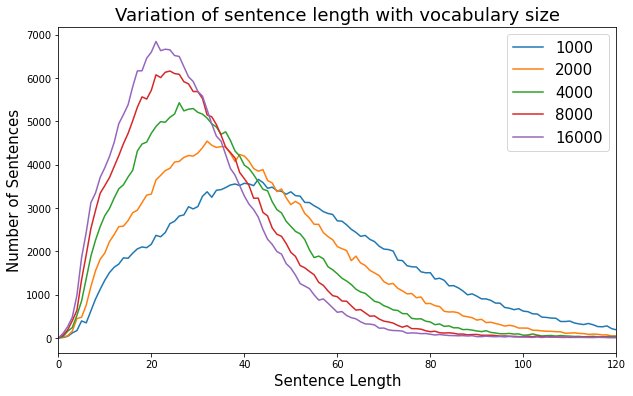
\includegraphics[width=\textwidth*5/8]{figs/length-vs-vocab-size.png}
    \caption{The distribution of sequence lengths w.r.t BPE vocabulary sizes(\textit{in the legend}). }
    \label{fig:sentence-length-vs-vocab-size}
\end{figure}
Through further investigation, it was concluded that because BPE is a greedy algorithm, when the vocabulary size is large, it will assign one subword to the frequently occurring words. Thus, leading to shorter sequences. Regardless of the computation boost owing to shorter sequences, it undoes most of the benefits described in the subsection \ref{bpe}. Moreover, with the help of the analysis conducted in the paper\cite{vocabsize}, the vocabulary size was set to \textbf{8000}.

\subsubsection{Sentence-Piece}

It provides many functions for subword tokenization like the one being used for this project, BPE. A benefit of using Sentence-Piece is that it takes raw files as its input. Consequently, to learn the vocabulary model, the previously generated dataset with a million sentence pairs is used in their raw text file format along with the following parameters:
\begin{itemize}
    \item \lstinline{model_type}: to specify `BPE'
    \item \lstinline{model_prefix}: to specify the name of the model. Used later in the pipeline
    \item \lstinline{vocab_size}: set to 8000
    \item \lstinline{character_coverage}: set to 1.0 to specify complete character coverage.
    \item \lstinline{pad_id}: the index reserved for the padding token is set to 3 since the default(-1) causes problems further down the pipeline because the model is expecting a Tensor with indices and -1 is not an index.

\end{itemize}
The Sentence-Piece model only needs to train once. Whenever it is needed to tokenize or detokenize, it just needs to be loaded into our program by using the \lstinline{model_prefix}.

\begin{figure}[H]
    \centering
    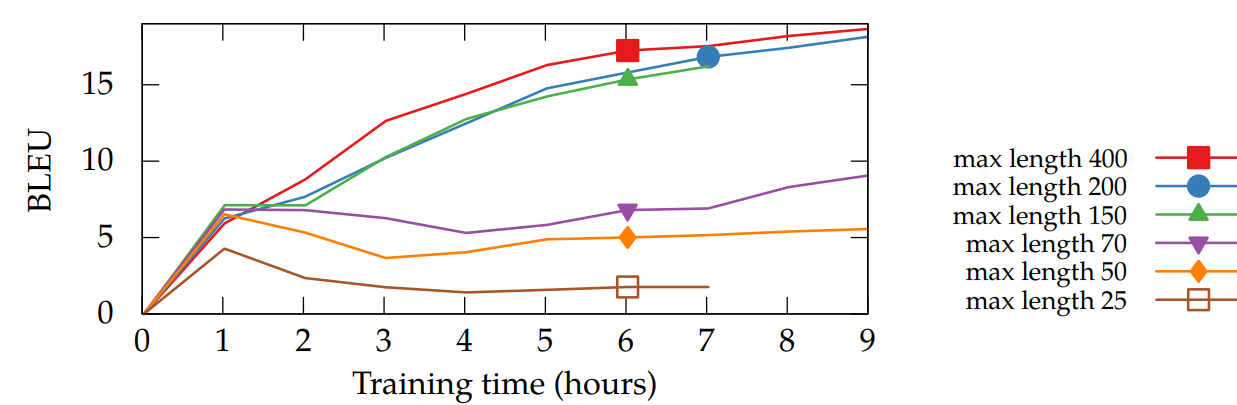
\includegraphics[width=0.9\textwidth]{figs/fig4frompaper-trainingtips.PNG}
    \caption{The \bleu scores over time for different maximum length thresholds \\(from the paper\cite{training-tips})
    % The graph shows the effect of various maximum length values on the performance verses time the model was trained (from the paper\cite{training-tips}).
    }
    \label{fig:figure-4-from-paper}
\end{figure}

\subsubsection{Filtering Long Sentences}
Once the vocabulary model has been used to tokenize the sentence into a sequence of IDs (indices in the vocab dictionary), the sequence's size needs to be checked to make sure it is below a threshold. It is impossible to train on very long sentences because the computation graph computed during the backpropagation is so huge(\textit{more than 15\textsc{gb}}) that it leads to an Out-Of-Memory (OOM) Exception.
\\\\
The threshold for maximum length introduces another hyperparameter that must be set to an appropriate value; else, it can completely wreck the training process. In the article\cite{training-tips}, the authors examined and reported the figure \ref{fig:figure-4-from-paper}. It depicts that setting max length to a small value like below 70 will adversely affect performance as the BLEU scores stagnate at around 5-10.
\\\\
We want the maximum-length threshold to be as high as possible to allow for maximum generalisability. That's because training on shorter sequences hampers performance on longer sequences, even if we are using Transformers. This is a result from the \textit{Unit of assessment: Deep Neural Networks}. For this project, the maximum-length was chosen to be 150.
% It is suggested that the highest possible maximum length should be used. This is essentially a trade-off between the complexity arising from the extensive computation graph calculation and generalisability.
% A result from the \textit{Deep Neural Networks (Unit of Assessment)} which is quite pertinent here is that sequence models do not generalise to longer sequences if they were exposed to only short sequences during the training process.

% \begin{figure}[]
%     \centering
%     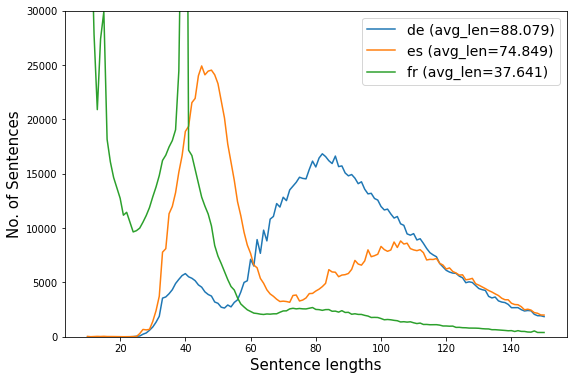
\includegraphics[width=\textwidth*5/8]{figs/length-distribution-across-languages.png}
%     \caption{Graph shows the distribution of sentence length after tokenization using BPE. %The sentences lengths chosen for each sentence pair was the maximum of the source/target sequence after tokenization with BPE(vocabulary size 8000).
%     }
%     \label{fig:distribution-across-languages}
% \end{figure}

\subsubsection{Padding}
After tokenization and removing the longer sentences, padding tokens are added to the source and target sequences to ensure they are the same length. Keeping the length of each sequence pair the same helps to calculate the overall tokensize and therefore, aids in building batches.
%Moreover,  in a PyTorch Tensor, the size of each sequence in a batch should be the same; else, it leads to an Error.
Finally, each pair is added to a Bin based on their length, hence, extra padding tokens may be added to make sure they are the correct length for that bin. Different strategies for constructing bins is covered in the next subsection \ref{bins}.

% After tokenization and removing the long sentences, padding needs to be added to the remaining sequences to make them the appropriate length. The length is decided by the structure of the \textbf{bins} described below (in subsection \ref{bins}).
% %It must be ensured that the source/target sequence have the same number of tokens.
% The sequences need to be the same size because it helps calculate the overall tokensize of each sentence pair, which aids in calculating batch sizes.

% Therefore, keeping both the source/target sequences the same length aids in decreasing the complexity of the batching algorithm.



\subsection{Bins}
\label{bins}

\begin{table}[]
\centering
\resizebox{0.7\textwidth}{!}{%}
\begin{tabular}{p{2cm}p{2cm}p{2cm}p{2cm}p{2cm}}
\toprule
\multirow{2}{*}{Tokensize} & \multirow{2}{*}{Raw} & \multicolumn{3}{c}{Effective} \\
\cmidrule(l){3-5}
&   & na\"ive    & big      & small  \\
\midrule \midrule
1024 & 14.4k & 1.5k & 7.4k & 13.4k   \\
2048 & 14.5k & 1.4k & 7.1k & 13.6k   \\
3072 & 15k & 1.5k & 7.4k & 14k \\
4096 & \textbf{15.5k} & 1.4k & 7.3k & \textbf{14.4k} \\
\bottomrule
\end{tabular}}
\caption{The \textbf{Raw} and \textbf{Effective} throughput for different tokensizes and batching% methodologies that were discussed above. It was also found that 30\% of tokens in each batch for the Na\"ive approach were actual tokens (not pads). Similarly for the Big and Small approach it was 91.8\% and 99.8\% respectively
}
\label{table:raw-and-effective-throughpu}
\end{table}

This section details a method adopted to increase efficiency by altering the scheme in which padding tokens are added to the sequences. When we pass a sequence to the Transformer, an equal amount of computation is performed on the actual tokens and the padding tokens.
\\\\
Consider a na\"ive approach where all the sequences are padded to be maximum length. It will require a basic batching algorithm that can assign any sequence to a batch. However, considering the above statement, a large portion of the computation will be wasted. Consequently, in a short experiment it was found that in this method only 10\% of the overall computation is useful. In other words, to increase the throughput of the Transformer in training, the number of padding tokens in each sequence must be minimised.
\\\\
Keeping this in mind, the first approach  was to use bins of some fixed size like \\$\text{bins} = [32, 40, 48, 56, 64...152]$. This method is referred to as ``big''. In this method, each pair is assigned to the bin corresponding to $b$ size, provided the source and target sequence lengths are less than or equal to $b$, where $b \in \text{bins}$. The two sequences then have padding tokens added to them so that their size equals $b$. This method does better than the na\"ive approach but only about 47\% of the overall computation is used on actual tokens.
\\\\
Considering how well the first approach faired against the initial na\"ive approach, the next and final (\textit{``small''}) approach was to use bins of width one. To achieve this, the source/target sequence was padded so that they were the same length and then placed into the bin corresponding to their length. Most importantly, most of the computation involved in this strategy was used on actual tokens (85\%). All of the these steps are present to boost efficiency of the translation model.
%and reduce the minimum size of the bins since examination revealed there were tons of shorter sequences in French, i.e. $\text{bins} = [10, 11, ... \text{max length}]$. %As shown in Figure \ref{fig:distribution-across-languages}, French peaks at around 20 and 40 attaining a value of 70K sentence-pairs. Finally, this approach had the highest effective throughput and about 85\% of the resources were used to process actual tokens.

% Please add the following required packages to your document preamble:
% \usepackage{multirow}


% random batches of some average length


\section{Transformer Architecture}
\label{transformer-architecture}
After the preprocessing step, the data is ready to be fed into the translator for training. In this section, various parts of the architecture are discussed and how they were implemented in PyTorch. A diagram of the Transformer architecture can be seen in Figure \ref{fig:transformer-architecture} towards the end of the section.
\\\\
\begin{specialfootnote}
For this project, the Transformer(\textit{Base}\footnotemark[2]) architecture was used. It is smaller and does not perform as well as the Transformer(\textit{Big}\footnotemark[2]) architecture, but it meets the computational restrictions.

\footnotetext[2]{From the paper\cite{transformers}, \textit{Big} has twice the model dimension ($d_{model}=1024$), feed-forward dimension ($d_{ff}=4096$) and attention heads ($h=16$)}
\end{specialfootnote}


\subsection{Embedding layers}
\label{embedding-layers}

A batch of sequences is passed to the Transformer in the form of a matrix with the shape [B x S], where B is the number of sequences in the batch and S is the sequence length. The words are one dimensional token IDs and need to be converted to embedded vectors with a size equal to the model dimension ($d_{model} = 512$ for \textit{Base}). \lstinline{torch.nn.Embeddings} was used to implement this layer which learns the embeddings for each token. The Embedding Layer is an integral part of the Transformer because the embedded vectors are critical to the attention sublayers, which learn to exploit the embeddings to understand the relationships between words.

\subsection{Positional Encoding}
\label{pe}
Each operation in this architecture is either point-wise (like embedding or feed-forward) or treats the sequence as a set (like attention or linear norm). Therefore, the model does not know the relative or absolute position of the token in a sequence.  Out of the many ways to overcome this issue, the authors in\cite{transformers} suggested a point-wise addition of sine and cosine functions with the wavelength in a geometric progression commencing at $2\pi$ to $10000 \cdot 2\pi$. These are formulated as follows:
\begin{align*}
    PE_{p, 2i} &= sin(p / 10000 ^ {(2i/d_{model})})\\
    PE_{p, 2i+1} &= cos(p / 10000 ^ {(2i/d_{model})})
\end{align*}
where $p$ is the position of the token in the sequence and $i$ is the dimension. These Positional Encodings (PE) are added point-wise to the embedding vectors.

During implementation with PyTorch, the matrix with 150 x 512 items was turned into a PyTorch buffer. Doing so allows PyTorch to track and store the PE as parameters. They move between the CPU and GPU like the features, but they are not part of the Stochastic Gradient Descent (SGD).

\subsection{Multi-Head Attention}
\label{attention}

The self-attention described in Section \ref{background} \nameref{background} is the basic version of Self-Attention. This operation has been enhanced by three keys advances. These are using Query, Key and Value matrices, scaling the dot product and using multiple-heads.

\subsubsection{Queries, Keys \& Values}

Recall, every input-vector $x_i$ is utilised in 3 different ways in the self-attention operation:
\begin{itemize}
	\item[\textbf{Q-}] Query:  it is utilised to calculate the weights for its output vector $y_i$
	\item[\textbf{K-}] Key:  it is utilised to calculate the weights of all the output vectors $y_j$
	\item[\textbf{V-}] Value:  it is included in the final weighted sum to get the output vectors after the weights have been ascertained.
\end{itemize}

In the basic version, we utilise the input vectors for all these three roles of Query, Key and Value. While in this version, learnable parameters are injected in the form of matrices $W_q$, $W_k$ and $W_v$ to build separate vectors for each role which can help form better output vectors. These matrices are built using \lstinline{torch.nn.Linear} (which are fully connected neural networks.)

\[
    q_i = W_q x_i
    \;\;\;\;\;\;\;\;\text{ and }\;\;\; \;\;\;
    k_i & = W_k x_i
    \;\;\;\;\;\;\;\;\text{ and }\;\;\;\;\;\;
    v_i = W_v x_i
\] \[
    w'_{ij}  = q_i^\top k_j
    \;\;\;\text{ then }\;\;\;
    w_{ij} = \text{softmax}(w'_{ij})
    \;\;\;\text{ then }\;\;\;
    y_i = \sum_j w_{ij} v_j
\]


\subsubsection{Scaled-Dot product}

Since there is a softmax operation involved, the large values that appear may completely ruin the results after this operation and cause the learning to come to a complete halt.
For an vector in $\mathds{R}^k$ with all the values equal to $a$. The Euclidean length is $\sqrt{kc}$, and thus, adding more dimensions increases the length of the average vector. Therefore, the scaling factor is decided to be $1/\sqrt{d_k}$.
Where the size of the Query and Key vectors are $d_k$ and the size of the Value vectors is $d_v$

\[ w'_{ij} = \frac{q_i^\top k_j}{\sqrt{d_k}} \]



\subsubsection{Multi-head Attention}

The current implementation can, over time, learn to pick up on how each word in the sequence is related to another. It is obvious that all of these relationships get summed into one and arguably makes it more complex and, therefore, more troublesome to learn. For example, in the sentence:
\begin{center}
    \changedFont{ ``Ana took chocolates from Bob"}
\end{center}
Here \textit{"took"} is related to ``Ana", ``Bob" and ``chocolates", albeit in entirely different ways: \textit{Ana} is someone who takes; \textit{chocolate} is the something that is taken and \textit{Bob} is the one who gives. This is just one example of the complex relationships that need to be learnt with a single self-attention operation.
\\\\
A simple solution is to use multiple self-attention operations (instead of just one) and combine the results. These are called \textbf{attention heads} and indexed them by $(\cdot)^r$. Consequently, $W_q$, $W_k$ and $W_v$ turn into $W^r_q$, $W^r_k$ and $W^r_v$

\begin{figure}[H]
    \centering
    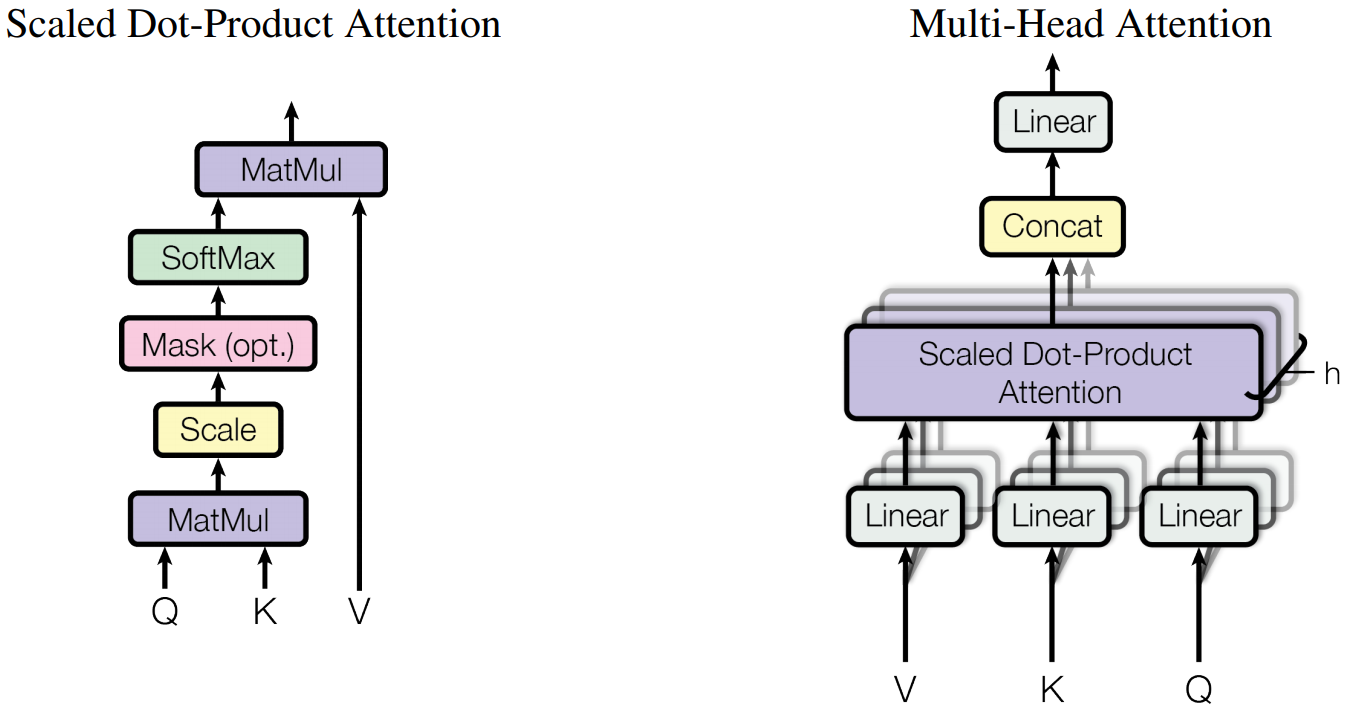
\includegraphics[width=0.8\textwidth]{figs/multihead-attention.PNG}
    \caption{Displaying the Scaled Dot Product (left) and Multi-head Attention mechanism (right) with multiple attention layer running in parallel. Taken from the paper\cite{transformers}}
    \label{fig:multi-head-attention}
\end{figure}


\subsubsection{Implementing Multi-Head Attention}

There are two ways to implement the Multi-head Attention mechanism. These are the Narrow and Wide approaches. The Narrow Multi-head attention approach was chosen because it is less computationally intensive and moreover, the method that was used in the paper\cite{transformers} as shown in Figure \ref{fig:multi-head-attention}. To explain it further, suppose our input vectors have a dimensionality of 512 as before and the number of attention heads we are using is 8. In the Narrow Multi-head attention approach, our matrices $W^r_q$, $W^r_k$ and $W^r_v$ will have the size 512 x 64. This will transform the input vector into 8 vectors of 64 width and at the end, we will be simply concatenating the output from each head to get back to the size of 512.
\\\\
Accordingly, the Query, Key and Value matrices were built as \lstinline{torch.nn.Linear} layers with input and output size set to the same value ($d_{model}$). After the query, key and value vectors are calculated, they are transformed from a size of [B x S x $d_{model}$] to [B x S x H x $d$], where B and S are as defined before; H is the number of heads; and $d$ (=$d_{model}$/H). Then we follow the self-attention methodology as described before.

% \\\\
% \textbf{Finally}, without getting lost in the details of the multi-head attention mechanism, it suffices to remember moving forward the broad strokes but remember it is the most important component.



\subsection{Position-Wise Feed Forward Networks}
\label{fc2}
After the attention layers, both the Encoder and decoder contain a two-layer point-wise Feed-Forward network which performs a linear transformation with a ReLU (Rectified Linear\cite{relu}) activation in between them and an inner-layer dimensionality of $d_{ff}=2048$.
\\\\
A single layer point-wise feed-forward Network is used at the end and applied to the decoder's output. It takes the decoder's output and transforms the vectors from $d_{model}$ to vocabulary size, from 512 to 8000. Lastly, we apply a softmax layer and this gives us the output probabilities for each word at each index.

\subsection{Regularisation}
\label{regularization}
There are two regularisation methods applied: Residual links and dropout.
\\\\
\textbf{Dropout}\cite{dropout} is ignoring some randomly chosen nodes. It is used during training for deep models to ensure that the model does not overfit the training set. It also ensures that the model generalises better to unseen data. The dropout rate was set to 0.1
\\\\
\textbf{Residual connections}\cite{residual-connections} are adding the input of a sublayer to the output from the sublayer:
\[ y = x + \text{SubLayer}(x)\]
First used to build Deep Convolutional Networks for image classification. The reason they work is that
unlike traditional models, the data path through residual networks varies in length and allows the model to work as an ensemble of networks. Non-linear activations naturally cause the gradients to explode or vanish for very deep networks. The addition of these `skip connections' allows the gradient to flow through directly and undercut the non-linear activations' problem.

\subsection{Layer Normalisation}
\label{layer-norm}
Between each sublayer (multi-head attention and feed-forward) layer normalisation is carried out. Layer normalisation ensures that there is a smoother gradient, faster training and allows for better generalisation.
Layer normalisation is vital; however, when it is carried out is equally relevant, i.e. after (Eq 3.1) or  before (Eq \ref{eq:norm-before}) every sublayer. A significant problem during the training process was that the model developed with the normalise-after methodology would not converge at all. After spending hours experimenting/testing each of the model's components extensively, the solution was found thanks to the explanations in the paper\cite{layernorm}. The authors advised using the normalise-before method because it diminishes the dependence of the output on the residual branches. However, they did criticise the normalise-before method as it did not produce models of the same quality as normalise-after. Considering this trade-off, the normalise-before methodology was selected.

\begin{align}
    y &= LN(x + \text{SubLayer}(x)) \\
    \label{eq:norm-after}
    y &= LN(x) + \text{SubLayer}(LN(x))
    \label{eq:norm-before}
\end{align}



\subsection{Encoder and Decoder}
\label{enc-dec}
After the indices are converted into embeddings and the positional encodings are attached. This input is now handed over to the Encoder \& Decoder where the bulk of the computation takes place. Their structure is displayed in the Figure \ref{fig:transformer-architecture}

% The Encoder/Decoder in the Transformer is built using multiple identical layers, further elaborated upon below. The output from each Encoder/Decoder layer is passed directly to the next with the same masks.

\begin{description}
\begin{specialfootnote}
\item[Encoder Layer]
Each Encoder layer comprises two main sublayers, the multi-head attention and the point-wise feed-forward operation with a layer normalisation before each layer and residual connections across each sublayer. The encoder takes as its input the source sequence/batch and the padding mask\footnotemark[8]. The output is the context for the source sequence that is passed to the Decoder.

\begin{figure}[H]
    \centering
    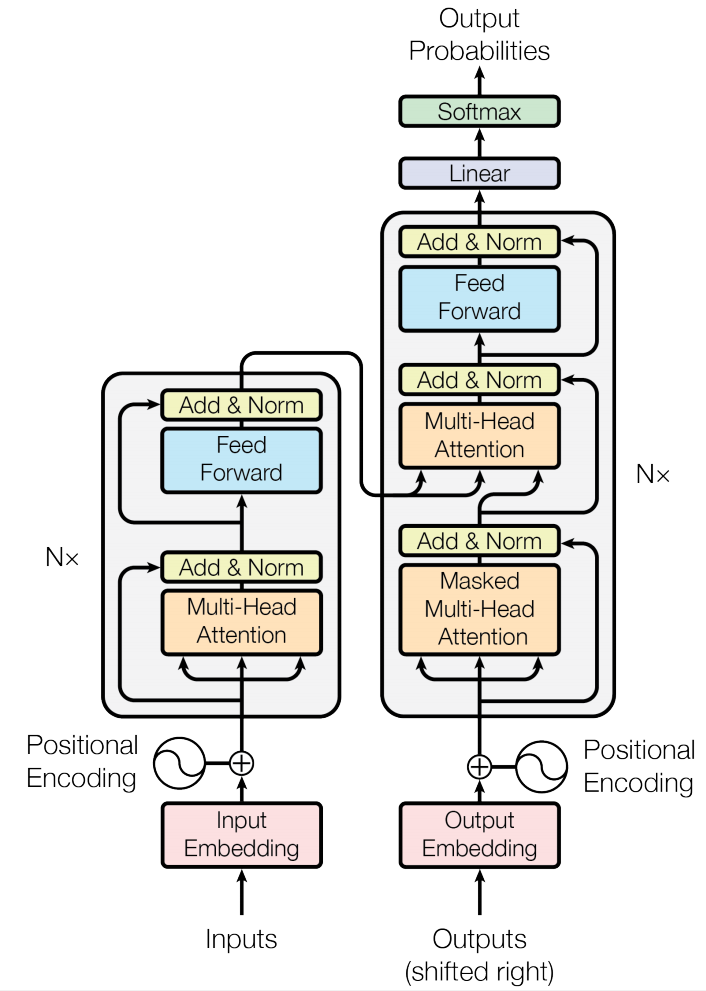
\includegraphics[width=\textwidth/2]{figs/transformer-architecture.PNG}
    \caption{The Transformer architecture from the paper\cite{transformers}}
    \label{fig:transformer-architecture}
\end{figure}

\item[Decoder Layer]
Each decoder comprises three main sublayers: the multi-head attention layer, point-wise feed-forward layer and an encoder-decoder attention layer. The encoder-decoder attention layer is a multi-head attention layer with the Keys and the Queries set to the Encoder's output. The input to the Decoder is the Encoder output, the target sequence that has been generated (during evaluation) or the target sequence (during training) along with the source padding mask\footnotemark[8] and a combined mask\footnotemark[8] containing the target padding mask\footnotemark[8] and the no-peak-mask\footnotemark[8].

\footnotetext[8]{More information about masks including their purpose, their structure and how they are constructed is covered in \ref{training-step}}
\end{specialfootnote}
\end{description}



\section{Training}
\label{training}\
After covering the architecture of the Translation model, this sections aims to describe the choice of hyperparameters, the training algorithm, the text generation algorithm used and the model validation algorithm carried out periodically.

\subsection{Hyperparameters}
\label{hyperparameters}

\textbf{Dataset size}: A larger dataset size has been shown to improve the translation model's quality. However, as discussed in Section \ref{dataset-clipping}, this was set to one million sentence pairs because of the time and memory restrictions.
\\\\
As discussed in the subsection \ref{tokenization}:\\
\textbf{Vocabulary size} was chosen to be 8000.
\\
\textbf{maximum length} was chosen to be 150.
\\\\
\textbf{Layer Normalisation} was set to before each sub-layer within the encoder/decoder units, as discussed in the subsection \ref{layer-norm}.
\\\\
\textbf{Batch size} for a transformer is often referred to as token size. Token size is defined to be the product of the number of sequences and the length of the sequence. In the first assignment \textit{Deep Neural Networks Unit of Assessment} an experiment on the effect of different batch sizes and learning rates was conducted. It shed light on the fact that having a larger batch size leads to faster convergence, provided that the learning rate is reasonably low. Similar conclusions were reached in the paper\cite{training-tips}, which showed that having a larger batch size raises not only the throughput but also improves the \bleu score. Nevertheless, the maximum number of tokens used on Google Colab's GPU was limited because of the memory restrictions and was approx 7500.
\\\\
After weighing all of these findings, the batch size/token size was set to $4096$. A power of two was used, keeping in mind the GPUs' architecture, which tends to have some power of 2 execution units. Hence, when work gets scheduled, we will not have too many execution units sitting idle and thus, improve the throughput.
\\\\
\textbf{Optimizer hyperparameters} following the implementation from the paper\cite{transformers}, the Adam optimizer\cite{adam} maintains a per-parameter learning rate using adaptively estimated moments (1st and 2nd order). It uses $\beta_1 = 0.9$ for the exponential decay rate for the 1st moment and $\beta_2=0.98$ for the exponential decay rate for the second moment along with $\epsilon=10^{-9}$, a small number, to prevent division by zero. The learning rate was first increased linearly for the \textit{warmup\_steps} and then decreased proportionally to inverse square-root of the number of steps:
\[ lr = d_{model}^{-0.5} \cdot min (\text{step\_num}^{-0.5}, \text{step\_num} \cdot \text{warmup\_steps}^{-1.5}) \]
This idea was introduced in\cite{transformers} and the choice of \textit{warmup\_steps} was taken from the paper\cite{training-tips}, which concluded that using less than 12k \textit{warmup\_steps} can lead to divergent training. Consequently, it was set to \textbf{16k}.
\\\\
\textbf{Transformer Hyperparameters} These hyperparamters were chosen match the \textit{Base}-architecture in the paper\cite{transformers}. \\
{Model Dimensions ($d_{model}$)}: \textbf{512}
\\
{Number of attention heads ($h$)}: \textbf{8}
\\
{Number of encoder-decoder layers ($N$)}: \textbf{6} each
\\
{dropout}: \textbf{0.1}
\\
Finally, out of the two Narrow and Wide multi-head attention, described in the subsection \ref{attention}, the \textbf{Narrow} version was implemented. All of these hyperparameters ensure that we do not reach an Out-of-memory exception and that we are maximising the efficiency of the GPUs used.


\subsection{Training step}
\label{training-step}
\subsubsection{Batching}
% \begin{figure}
%     \centering
%     \begin{lstlisting}
%     def batch(bins: Dict[int, List[List[int]]], tokensize: int):



%     \end{lstlisting}
%     \caption{Batching algorithm \red{should I include this?}}
%     \label{fig:batching algorithm}
% \end{figure}
The batching algorithm is implemented as a generator\footnote{Generator Functions allows us to declare a function that behaves like an iterator, i.e. it can be used in a for loop.} function in Python in order to simplify the code. We begin by shuffling the order of the sentence pairs in each bin. Then chooses a random bin and builds a batch by selecting the required number of sequences from the bin. \\
Thus, the batch iterator returns two 2d arrays of the shape [$token size // b$, $b$], one each for the sequence in the source and target languages. \\
Where the bin size is $b$ and the token size/batch size is $token size$, then the required number of sequences is the output of the integer division of the two: $token size//b$.



\subsubsection{Inputs and Outputs}
The 2d-arrays from the batch iterator need to be transformed into a compatible form with the training step. The source array gets converted into a \lstinline{torch.LongTensor} and is moved onto the GPU.

\begin{lstlisting}
    target_tensor_input = target_array[:, :-1]
    target_tensor_output = target_array[:, 1:]
\end{lstlisting}

 For the target array, first a beginning-of-sequence character \lstinline{<bos>} \& a end-of-sequence character \lstinline{<eos>} is added at the appropriate position. The above code represents the transformations carried out on the target array.
Then for each sequence in the batch, all but the last item is used to build the target tensor.
The expected output from the Transformer is set to a \lstinline{torch.LongTensor} constructed from the target array with every item in each sequence except for the first one.
\\\\
Consequently, the training algorithm is designed such that, for every position in the input target tensor, we expect to see the following word in the sequence to have the highest probability in the target predictions. \\
The benefits of the immense parallelizability of Transformers can be seen here. Usually, sequence models recurrent architecture require that the sequence is passed serially for both during the training step. However, with Transformers, the entire sequence moves through the model in parallel.

\subsubsection{Masks}
Two types of masks need to be employed to ensure that the attention operation works as expected.

Firstly, perhaps the most obvious one, that is the \textbf{padding mask}. Pads were added to the source and target sequence to ensure they were the same length. These pads would be considered as part of the sequence if they were removed using masks. To build the padding mask for the sequences, the following code is used.
\begin{lstlisting}[label=padding-code]
    padding_mask = (sequence != pad)
\end{lstlisting}

Another mask required is the \textbf{no peak mask} that will ensure that the decoder can not peak at the following (future) words when making its predictions. To construct it the following code is used:
\begin{lstlisting}[label=nopeak-mask-code,caption=No Peak Mask generator]
def nopeak_mask(size):
    np_mask = np.triu(np.ones((1, size, size)), k=1)
    np_mask =  torch.from_numpy(np_mask) == 0
    return np_mask

# output for size=3
# [[[1., 0., 0.],
#  [1., 1., 0.],
#  [1., 1., 1.]]]
\end{lstlisting}

Here, an upper triangular matrix is constructed and then 1s and 0s get flipped to produce a matrix, as shown above. This nopeak mask is combined with the padding mask discussed before to form the mask for the target tensor.

\subsubsection{Mask Application}
The mask is applied before the softmax operation. We add a large negative number ($-10^9$) to the positions we want masked (indices that have a 0 in the mask). Thus, when the exponentiation takes place in the softmax, these values are suppressed to zero.
%In order to apply the mask, before the softmax operation, $-10^9$(a large negative number) is added to all those positions where the mask is 0. During the softmax operation, the element-wise exponentiation causes these values to be suppressed to zero.

\subsection{Text Generation}
\label{text-generation}
Once a model has been trained. It will need to generate text.
In an ideal world, we would search all possible sequences before returning the sequence with the highest probability. Nevertheless, resource restrictions mean that we have to settle for heuristic-based search algorithms for text generation like Beam Search\cite{beam-serach-paper} or Greedy search.
\\\\
The structure of any text generation algorithm is to generate words in steps, i.e. one `word' at a time. With Transformers, first, the encoder output is calculated by passing the source sequence through the transformer-encoder as we did in training. The encoder output is used as the context/memory to inform the next generation and is passed to the transformer-decoder. At the start, only the beginning-of-sequence word \lstinline{<bos>} is passed to the decoder. As words are generated, all of them are used to inform the next word to be generated. Recognising that the predictions will be a probability distribution on the entire vocabulary at each step, consider two implementations of text generation algorithms attempted in the project.

\subsubsection{Greedy Search}
To understand how Beam Search works, it helps to look at a Greedy algorithm which is essentially a Beam search with a width of 1. Moreover, it is an easy to execute and quick algorithm that was used initially to evaluate/test the model before moving onto Beam Search. In this algorithm, the most likely word, i.e. the word with the highest value after the final softmax operation, is chosen as the predicted word.
\\\\
It is trivially straightforward why this algorithm does not do too well. Since the word probabilities might not be accurate initially, the first few words generated may be incorrect. This form of error piles up at each step as we move through the sequence.

\subsubsection{Beam Search}
Beam Search is a pruned version breadth-first-search. There is some preset search width commonly referred to as $k$. The most significant difference from the Greedy Search is that we hold the top-k most likely words for each step. Hence, there is only one sequence at the start, and after considering 8000 words (vocabulary size), $k$ words are chosen, which form the $k$ sequences we will consider for the next word. In the next step and all subsequent steps, $k$ sequences are used to generate $8000 \cdot k$ words from which again $k$ words are chosen. The commonly used $k$ is about 5 to 10, and for the evaluation and translation steps, $k$ was set to 10. Finally, for all the finished sentences a length penalty is tacked on to ensure that we select longer sentences.


\subsection{Model Evaluation}
\label{model-evaluation}
After each epoch
%\footnote{refer to Section \ref{background}}
the model is tested on a small parallel corpora built with the test sets from WMT. The corpora contain about 2000-3000 sentence pairs. For each sequence, the model produces a translation using the Beam Search/Greedy Search described above in subsection \ref{text-generation}.
\\\\
Following translation, \bleu scores were calculated (using Sacre\bleu) and stored.
%For the first three epochs, the scores are just stored. Following that,
After the first three epochs, the new \bleu score is compared to the average of the last three, and if there is no substantial improvement in the scores, then the training is stopped. A substantial difference here refers to an increase of $> 0.01$, i.e. the difference between the new score and the moving average must be $> 0.01$.

% \red{mention which ones exactly}

\section{Pipeline Overview}
\label{pipeline-overview}
This section describes all the work involved in the pre-processing, translation, summarisation and post-processing involved in the final evaluation step.

\subsection{Pre-Processing}
\label{preprocessing}
These steps were followed to collect all the relevant data before moving onto translation and summarisation.
\begin{enumerate}
    \item Load the JSON files (GV-snippet and GV-crowd)\footnote{refer to Sub-Section \ref{functional-requirements}}.
    \item Filter both the JSON objects so that they only contain the entries comprising articles in the required source language (de/es/fr). Checking the language also helped to weed out a lot of unnecessary text like links or extra text.
    \item Join the JSON objects into one. Here, the auxiliary information in both JSONs was found to be the same and thus, the snippet summary was copied into the current filtered GV-crowd JSON and under a new key.
    \item The final step involved reading the articles in both the source and target language, provided as markdown files.
\end{enumerate}

\subsubsection{Processing the markdown article}
The markdown files had sentences separated by a newline character which reduced some processing required.
%The markdown articles for all languages were such that there were two newline characters between each of the sentence. Hence, reducing the amount of processing needed to get down to the sentence level partition.
Moreover, the English articles were quite clean whereas, the articles in French (fr), Spanish (es) and German (de) contained hyperlinks and, most importantly, extra text like \\
\changedFont{"Compártelo: Twitter Facebook Reddit google plus"}\\
Which in Spanish means: \\
\changedFont{"Share on Twitter Facebook Reddit google plus"}\\
These had to be cleaned before being fed the source articles into the translator. French and German had similar problems, but they were not as frequent, and therefore, nothing was done for them.

\subsection{Translation}
\label{translation}
The checkpointed models were loaded and then the positional encodings were updated to have a maximum length of 300 to ensure that the model can handle longer sequences during the inference step.
Using Beam Search (described above in the subsection \ref{text-generation}), each sentence in the source language is translated into the target language (English). The translated sentences are then collected into one line and written to a file, and ready to be summarised.
\\\\
Once all the articles were translated, Sacre\bleu was used to calculate the \bleu score for the translation and consequently, stored as well.
\newpage
\subsection{Summarisation}
\label{summarisation}
As described in the \ref{auto-text-summarisation}, the pre-trained summariser following the Bottom-Up Abstractive architecture is used. %Another benefit of using Jupyter notebook comes to light in this step: invoking shell commands within a for-loop in Python and using Python variables within the shell command.
The hyperparameters used for the generation are as follows:

\begin{description}
  \item[minimum length]: 35 (\textit{Ensures that the minimum length of the output summary is 35})
  \item[stepwise penalty]: A penalty that is applied at every step.
  \item[beta ($\beta$)]: 5 (\textit{ Parameter used for the Coverage Penalty})
  \item[coverage penalty]: applied (\textit{a penalty used to prevent the repeated attention to the same source word}).
  \[ cp(X, Y) = \beta \sum^{|X|}_{i=1}log\left(min\left( \sum^{|Y|}_{j=1} p_{i,j}, 1.0 \right)\right) \text{,} \] where $p_{i, j}$ is the attention probability of the jth target word $y_j$ on the ith source word $x_i$ and $|X|$ is the source length and $|Y|$ is the current target length.
  \item[alpha ($\alpha$)]: 0.9 (\textit{Parameter for the Length Penalty})
  \item[length Penalty]: ``wu''\cite{wu} applied (\textit{A penalty added on} \lstinline{<eos>} \textit{tokens that helps prioritise longer sentences.})
  \[ lp(Y) = \frac{(5 + |Y|)^\alpha}{(5 + 1)^\alpha} \]
  \item[Beam size]: 10 (\textit{The search width $k$ from subsection \ref{text-generation}})
\end{description}

% \begin{itemize}
%     \item minimum length: 35 (\textit{})
%     \item Penalties applied were: Stepwise penalty (\textit{}), Coverage penalty (summary) and Length penalty (wu).
%     \item beam size of 20
%     \item beta set to 5 and alpha set to 0.9
% \end{itemize}

\subsection{Post Processing}
\label{postprocessing}

% \red{needs work}\\
The evaluation's final step is to collect the hand-translated sentences and the machine-translated sentences together to calculate the \bleu score. After that the generated summaries are collected together and the mean \rouge scores are reported in the \textbf{Chapter \ref{evaluation} \nameref{evaluation}} (specifically \ref{baseline-results} and \ref{translate-then-summarize}) along with inferences we can draw from the results.


\newpage
\section{Repository Overview}
\phantom{.}


\begin{wrapfigure}{l}{0.4\textwidth}
    % \centering
    \includegraphics[width=0.4\textwidth]{figs/repo.PNG}
    \caption{Repository Structure}
    \label{fig:repository-structure}
\end{wrapfigure}

There are four main directories of the repository for this experiment. They are as follows:

\phantom{.}\\
\textbf{colab-notebooks/} This directory contains the two jupyter notebooks\footnote{Note: In the final submission these python notebooks were converted to `.py' files in accordance to the guidance on moodle} that were used on Google-Colab to run the experiments.

\phantom{.}\\
\textbf{data/} This directory contains all the relevant data that is needed to run the programs and all the data generated during the experiments. This directory is further subdivided into directories relevant to each source language (de, es, fr).

\phantom{.}\\
\textbf{eval/} The directory contains the GV-snippet \& GV-crowd json files along with the web-scraped articles. The scripts used during the evaluation step are also present in this directory.

\phantom{.}\\
\textbf{src/} This is the most important directory and contains the meat of the project. It contains the preprocessing, training and utility scripts along with the transformer architecture definition. Finally, there is an \fbox{opt.py} which contains a singleton class that is used to pass arguments around.




% \begin{figure}[H]
% \centering
% \fbox{%
% \begin{forest}
% for tree={
%     font=\ttfamily,
%     grow'=0pt,
%     child anchor=west,
%     parent anchor=south,
%     anchor=west,
%     calign=first,
%     edge path={
%       \noexpand\path [draw, \forestoption{edge}]
%       (!u.south west) +(15pt,0) |- node[fill,inner sep=2.5pt] {} (.child anchor)\forestoption{edge label};
%     },
%     before typesetting nodes={
%       if n=1
%         {insert before={[,phantom]}}
%         {}
%     },
%     fit=band,
%     before computing xy={l=25pt},
%     inner sep=1pt,l=10pt,l sep=10pt
%   }
% [dissertation-project/
%     [colab-notebooks/
%         [Evaluation.ipynb]
%         [Training\_step.ipynb]
%     ]
%     [data/
%         [de/] [es/] [fr/]
%     ]
%     [eval/
%         [gv/
%             [normalized/]
%             [gv-crowd.json]
%             [gv-snippet.json]
%         ]
%         [evaluate.py]
%         [preprocessing.py]
%         [translate\_articles.py]
%         [summarise\_articles.py]
%     ]
%     [src/
%         [opt.py]
%         [sub\_layers.py]
%         [text\_preprocessing.py]
%         [training.py]
%         [transformer\_layers.py]
%         [utils.py]
%     ]
% ]
% \end{forest}%
% }
% \caption{The diagram represents the repository structure that was developed.}
% \label{fig:repository-structure}
% \end{figure}


\chapter{Evaluation}
\label{evaluation}

\section{Success Criterion}
All of the success criteria set out for this project were met. The criteria for success as listed on the initial project proposal are as follows:
\renewcommand{\labelitemi}{$\checkmark$}
\begin{itemize}
    \item Translator has been implemented
    \begin{itemize}
        \item Transformer architecture implemented (\textit{Covered in Section \ref{transformer-architecture}})
        \item Preprocessing steps taken before training begins (\textit{Covered in Section \ref{pre-processing}})
        \item Trained models for de, es and fr (\textit{Covered in Section \ref{training}})
        \item Multiple checkpointed models used to generate translations (\textit{Covered in Section \ref{pipeline-overview}})
    \end{itemize}
    \item Summariser used to generate summaries (\textit{Covered in Section \ref{pipeline-overview}})
    \item Comparison between \bleu and \rouge scores. (\textit{Covered in this Chapter})
\end{itemize}\renewcommand{\labelitemi}{$\bullet$}

% \begin{itemize}
%     \item Preprocessing steps involving training the vocabulary, tokenization and forming bins. (\textit{Covered in Section \ref{pre-processing}})
%     \item Research, Understand and Build the Transformer architecture that will become the Translator models. (\textit{Covered in Section \ref{transformer-architecture}})
%     \item Training the models for the initially chosen languages (de, es \& fr).\\(\textit{Covered in Section \ref{training}})
%     \item Using translation models to translate the source articles from the GV dataset and then use a pre-trained summariser to summarise the \perftrans and the translation.\\ (\textit{Covered in Section \ref{pipeline-overview}})
%     \item Finally, quantitatively and qualitatively evaluating the \bleu and \rouge scores. (\textit{Covered in the following sections.})
% \end{itemize}

% \renewcommand*{\thefootnote}{\fnsymbol{footnote}}


\subsection*{Interpreting \bleu and \rouge scores}
In section \ref{evaluation-methods}, I have detailed how to interpret \bleu and \rouge scores. This subsection reiterates the important points to help understand the data in this section.

\bleu is a precision based metric which reports how similar the candidate translation is to the references provided. The main idea is that the closer a candidate translation is to the ``\textit{gold-standard}'' reference the better the quality, and therefore, the higher the \bleu score. In the following experiments the scores are reported out of 100.

In the case of \rouge, the \fone-scores are considered meaning that the scores reported express how similar the candidate and reference summaries are to each other. There are different categories of \rouge namely 1, 2, L \& W each of which use a different similarity metric. Like the \bleu scores these are also out of 100 and higher scores imply the summarization quality is better.


\section{Baseline Results}
\label{baseline-results}

% \begin{specialfootnote}


% % \renewcommand*{\thefootnote}{\arabic{footnote}}
% \end{specialfootnote}

% \subsection*{Baseline {\rouge} Scores}
Table \ref{tab:baseline-results} reports the Baseline/Upper-bound \rouge-\fone scores with the candidate summaries in the form of \textsc{First50} and the summary generated with \perftrans compared against the reference summaries in the form of the `\textit{snippet}' and `\textit{crowd}' summaries from the GV-dataset and for all the languages i.e. de, es and fr.

\begin{table}[H]
\centering
\resizebox{0.75\textwidth}{!}{%
\begin{tabular}{ccccccccc}
\toprule
 &
  \multicolumn{4}{c}{\rouge(\fone) GV-snippet} &
  \multicolumn{4}{c}{\rouge(\fone) GV-crowd} \\ \cmidrule(r){2-5} \cmidrule(l){6-9}
\multirow{-2}{*}{\textbf{BASELINE}} &
  1 &
  2 &
  L &
  W &
  1 &
  2 &
  L &
  W \\ \midrule
           & \multicolumn{8}{c}{\textbf{de}} \\ \cmidrule(r){2-5} \cmidrule(l){6-9}
\perftrans & 43.4 & 29.3 & 42.4 & 21.1 & 38.7 & 16.5 & 33.3 & 13.7 \\
\textsc{First50}    & 73.6 & 66.9 & 73.6 & 44.7 & 48.3 & 25.8 & 41.6 & 18.8 \\ \midrule
           & \multicolumn{8}{c}{\textbf{es}} \\ \cmidrule(r){2-5} \cmidrule(l){6-9}
\perftrans & 44.0 & 29.6 & 42.8 & 21.6 & 38.1 & 15.4 & 32.6 & 13.2 \\
\textsc{First50}    & 69.5 & 62.2 & 69.6 & 42.2 & 47.5 & 24.1 & 40.8 & 18.2 \\ \midrule
           & \multicolumn{8}{c}{\textbf{fr}} \\ \cmidrule(r){2-5} \cmidrule(l){6-9}
\perftrans & 42.0 & 27.2 & 40.5 & 20.3 & 36.8 & 14.2 & 31.1 & 12.4 \\
\textsc{First50}    & 68.5 & 61.1 & 68.8 & 41.8 & 47.0 & 23.4 & 40.1 & 17.8 \\
\bottomrule
\end{tabular}%
}
\caption{Baseline Results}
\label{tab:baseline-results}
\end{table}

% The results seen in the Table \ref{tab:baseline-results} is discussed here. We can view them as baseline or an upper-bound on the \rouge scores\\
The scores achieved by the baseline \textsc{First50}, which is made up of the first fifty words in the article's English version, performs much better when compared to any of the summaries generated. \textsc{First50} achieves a \rouge-2 \fone score of 0.6, which is very high
%for a \fone measure
and therefore reveals, that the two summaries must be very similar. This trend is observed in all the languages. As explained before, the snippet summary is the description of the article that was web-scraped. Hence, we can claim that snippet summaries are most likely excerpts of text taken from the start of the article.
%Hence, revealing that the description for the article provided very similar to the \textsc{First50} summary.
% Therefore, the description is made up of mostly the \textsc{First50} words in the article.
Therefore, I decided to ignore the snippet summaries for the next step.

% Moreover, we are trying to investigate the effect of translation quality on Summarisation quality.  The hyperparameters used for the summarisation model are not optimal. The hyperparameters were chosen with care and after much research. Nevertheless, an in-depth understanding of the exact summariser model is lacking. Hence, there is the possibility that the summariser's configuration is not the best for this experiment.  Thus, the summary generated using hand-translated articles, the \textit{gold standard},  should serve as a valuable Control. At the same time, it must be noted that the \rouge-$(1|2|L)$ scores are pretty close to the highest values that the progenitors achieved.
\\\\
The \rouge-\fone-scores for candidate \perftrans summary and reference: GV-crowd can be regarded as the maximum score or upper-bound that can be reached should the translation be perfect. None of the candidate summaries in the Translate-then-summarise category come close. The best scores are at around two-thirds of this value. Considering that the best translation models have a \bleu score of 26(es), 18.8(fr) and 16(de), this is the first evidence towards the hypothesis that the translation quality does affect the summarisation quality.



% \end{description}










%%%%%%%%%%%%%%%%%%%%%%%%%%%%%%%%%%%%%%%%%%%%%%%%%%%%%%%%%%%%%%%%%%%%%%%%

% \section{Discussion}
% \label{discussion}
% The main aim of this section is to discuss the results obtained and dissect the correlation between the \bleu scores and the \rouge scores along with other intricacies in this experiment similar to the experiments in the paper\cite{nguyen-daume-iii-2019-global}.










\section{Translate-then-Summarise Results}
\label{translate-then-summarize}
This section aims to discuss the results of the experiment and the trends that appear.
\\
Table \ref{tab:final-results} reports the different \rouge \fone scores and the \bleu scores for all the languages. These values are indexed by the Model Number which is the number of batches that have been digested by the model during the training process and within the parenthesis is the ratio of the model number with the epoch size. {\textit{Epoch Size}: is the number of training steps involved in one epoch.}
\\
Figure \ref{fig:rouge-v-bleu} displays the graph with \bleu scores in the x-axis and the different \rouge-(1, 2, L \&  W)-scores plotted with blue, orange, green and red respectively.

\phantom{.}\\
\begin{minipage}{\textwidth}
\begin{minipage}[c]{0.5\textwidth}
\flushleft
% \centering
\resizebox{\textwidth}{!}{%
\begin{tabular}{@{}ccc@{}}
\toprule
\toprule
\multicolumn{3}{c}{\textbf{de}, epoch size: 20.6k}                                                               \\ \midrule
\multirow{2}{*}{Model} & \multirow{2}{*}{\bleu} & {\textit{reference} GV-crowd} \\                                           & & \rouge-($1|2|L|W$)-f1 \\
5,000 (0.24) & 3.32 & $23.7\;|\;2.9\;|\;21.4\;|\;7.4$ \\
10,000 (0.48) & 12.03 & $30.5\;|\;6.9\;|\;26.1\;|\;9.5$ \\
20,000 (0.97) & 14.69 & $31.0\;|\;7.2\;|\;26.2\;|\;9.7$ \\
40,000 (1.94) & 15.66 & $31.8\;|\;7.6\;|\;26.3\;|\;9.8$ \\
60,000 (2.91) & 15.79 & $31.8\;|\;7.8\;|\;26.2\;|\;9.7$ \\
80,000 (3.87) & 16.14 & $31.4\;|\;7.7\;|\;26.5\;|\;9.9$\\
% 5,000 (0.12) & 3.32 & $24.7\;|\;4.2\;|\;23.0\;|\;8.3$ & $23.7\;|\;2.9\;|\;21.4\;|\;7.4$ \\
% 10,000 (0.24) & 12.03 & $32.9\;|\;10.2\;|\;30.2\;|\;11.7$ & $30.5\;|\;6.9\;|\;26.1\;|\;9.5$ \\
% 20,000 (0.48) & 14.69 & $34.8\;|\;11.2\;|\;31.2\;|\;12.4$ & $31.0\;|\;7.2\;|\;26.2\;|\;9.7$ \\
% 40,000 (0.97) & 15.66 & $35.6\;|\;12.4\;|\;32.3\;|\;13.0$ & $31.8\;|\;7.6\;|\;26.3\;|\;9.8$ \\
% 60,000 (1.45) & 15.79 & $36.4\;|\;13.0\;|\;32.7\;|\;13.2$ & $31.8\;|\;7.8\;|\;26.2\;|\;9.7$ \\
% 80,000 (1.94) & 16.14 & $35.6\;|\;12.4\;|\;32.0\;|\;12.8$ & $31.4\;|\;7.7\;|\;26.5\;|\;9.9$\\
\bottomrule
\end{tabular}%
}
% \caption{The evaluation outcome for German. Each epoch was made up of 20.6k training steps and overall there were 958,488 sentence pairs. }
% \end{table}

% \begin{table}[H]
% \centering
\resizebox{\textwidth}{!}{%
\begin{tabular}{@{}ccc@{}}
\toprule
\multicolumn{3}{c}{\textbf{es}, epoch size: 17.7k}                                                               \\ \midrule
\multirow{2}{*}{Model} & \multirow{2}{*}{\bleu}  & {\textit{reference} GV-crowd} \\
                     &                       & \rouge-($1|2|L|W$)-f1 \\
5,000 (0.28) & 4.11 & $24.1\;|\;3.5\;|\;22.4\;|\;7.8$ \\
10,000 (0.56) & 11.44 & $30.1\;|\;6.2\;|\;25.8\;|\;9.4$ \\
20,000 (1.13) & 20.52 & $32.4\;|\;8.0\;|\;27.7\;|\;10.3$ \\
60,000 (3.39) & 24.87 & $32.8\;|\;8.2\;|\;27.5\;|\;10.3$ \\
80,000 (4.52) & 25.02 & $32.9\;|\;8.2\;|\;27.7\;|\;10.4$ \\
110,000 (6.21) & 26.05 & $33.6\;|\;8.8\;|\;28.0\;|\;10.6$\\
% 5,000 (0.14) & 4.11 & $24.9\;|\;4.6\;|\;23.5\;|\;8.7$ & $24.1\;|\;3.5\;|\;22.4\;|\;7.8$ \\
% 10,000 (0.28) & 11.44 & $34.3\;|\;11.3\;|\;32.1\;|\;12.9$ & $30.1\;|\;6.2\;|\;25.8\;|\;9.4$ \\
% 20,000 (0.56) & 20.52 & $37.7\;|\;14.3\;|\;35.0\;|\;14.4$ & $32.4\;|\;8.0\;|\;27.7\;|\;10.3$ \\
% 60,000 (1.69) & 24.87 & $39.3\;|\;15.9\;|\;36.2\;|\;15.2$ & $32.8\;|\;8.2\;|\;27.5\;|\;10.3$ \\
% 80,000 (2.26) & 25.02 & $39.5\;|\;16.7\;|\;36.4\;|\;15.5$ & $32.9\;|\;8.2\;|\;27.7\;|\;10.4$ \\
% 110,000 (3.11) & 26.05 & $41.1\;|\;18.4\;|\;38.4\;|\;16.5$ & $33.6\;|\;8.8\;|\;28.0\;|\;10.6$\\
\bottomrule
\end{tabular}%
}

% \caption{The evaluation outcome for Spanish. Each epoch was made up of 17.7k training steps and overall there were 966,398 sentence pairs. }
% \end{table}

% \begin{table}[H]
% \centering
% \centering
\resizebox{\textwidth}{!}{%
\begin{tabular}{@{}ccc@{}}
\toprule
\multicolumn{3}{c}{\textbf{fr}, epoch size: 9.1k}                                                               \\ \midrule
\multirow{2}{*}{Model} & \multirow{2}{*}{\bleu}  & {\textit{reference} GV-crowd} \\
                     &                       & \rouge-($1|2|L|W$)-f1 \\
6,000 (0.66) & 3.09 & $23.4\;|\;3.2\;|\;21.3\;|\;7.4$ \\
12,000 (1.32) & 2.41 & $14.0\;|\;1.1\;|\;14.0\;|\;4.7$ \\
18,000 (1.98) & 12.29 & $30.0\;|\;5.9\;|\;26.0\;|\;9.4$ \\
33,000 (3.63) & 17.36 & $32.4\;|\;8.1\;|\;27.5\;|\;10.2$ \\
48,000 (5.27) & 18.85 & $33.2\;|\;8.6\;|\;28.0\;|\;10.4$ \\
72,000 (7.91) & 18.19 & $32.6\;|\;7.6\;|\;27.1\;|\;10.1$\\
% 6,000 (0.66) & 3.09 & $23.1\;|\;3.5\;|\;21.6\;|\;7.9$ & $23.4\;|\;3.2\;|\;21.3\;|\;7.4$ \\
% 12,000 (1.32) & 2.41 & $13.7\;|\;1.4\;|\;14.1\;|\;5.0$ & $14.0\;|\;1.1\;|\;14.0\;|\;4.7$ \\
% 18,000 (1.98) & 12.29 & $32.4\;|\;9.3\;|\;29.7\;|\;11.8$ & $30.0\;|\;5.9\;|\;26.0\;|\;9.4$ \\
% 33,000 (3.63) & 17.36 & $35.1\;|\;11.9\;|\;32.1\;|\;13.0$ & $32.4\;|\;8.1\;|\;27.5\;|\;10.2$ \\
% 48,000 (5.27) & 18.85 & $36.1\;|\;13.0\;|\;33.0\;|\;13.5$ & $33.2\;|\;8.6\;|\;28.0\;|\;10.4$ \\
% 72,000 (7.91) & 18.19 & $36.3\;|\;12.9\;|\;33.2\;|\;13.6$ & $32.6\;|\;7.6\;|\;27.1\;|\;10.1$\\
\bottomrule
\bottomrule
\end{tabular}%
}
\captionof{table}{Translate-then-Summarise results%: lists the \bleu score and the \rouge (1, 2, L \& W)-f1  scores. %The model number is the number of batches the model was exposed to during training. An epoch contains a fixed number of batches and therefore, the epoch number is defined to be the ratio of the model number to the number of batches, essentially telling us how many epochs have passed
}
\label{tab:final-results}

\end{minipage}
%\caption{The evaluation outcome for French. Each epoch was made up of 9.1k training steps and overall there were 988,639 sentence pairs. }
\qquad
\begin{minipage}[c]{0.45\textwidth}%
% \begin{figure}
    % \centering
    % \begin{flushright}

    \includegraphics[width=\textwidth]{figs/bleu-vs-rouge.png}
    % \end{flushright}
    \captionof{figure}{Variations of the different \rouge scores w.r.t. the \bleu scores for all languages}
    \label{fig:rouge-v-bleu}
% \end{figure}
\end{minipage}
\end{minipage}
\newpage



\subsection*{Models chosen}
For all three languages, I have tried to choose 3 models from the first/second epoch and they are expected to produce translation of poor quality because they have not been trained for long enough. The rest of the models are chosen from remaining checkpoints and the final model in each case is the last model to be checkpointed before the training was stopped.



\subsection{{\bleu} Scores}

% \subsubsection{\bleu Scores achieved}
Out of the models trained, Spanish (es) appears to perform the best, having the maximum \bleu score of 26.05, followed by French (fr) at 18.85 and then German (de) at 16.14. Spanish does the best, however, it took the most time to reach convergence as well. Because it took the longest, it reflects that Spanish is the most different to English out of the three languages chosen. Further, I speculate that the models could have performed better if they were trained longer rather than training till convergence.
%it is quite similar \red{spanish is least similar to english} to English, with only a few major differences, like adjectives before nouns.


French is also very close to English. However, when the parallel corpora were constructed for French, it appears to have ended up with shorter sentences.
French was the first languages I trained and I discovered that the French dataset had too many short sentences and an average length of 37 compared to more than 70 for German and Spanish. Thus, as described in subsection \ref{tokenization}, the model needed to see longer sequences to perform well.
%As shown in Figure \ref{fig:distribution-across-languages}, French had an average length of 37, half that of Spanish. Because the translation model needs to see long sentences to perform better, the French model suffers.
Sadly, this was discovered when it was too late to make a change. Nevertheless, it took a similar number of training steps to reach convergence.


Finally, German performs worst and that is the general trend seen in most papers where German is lagging behind other languages like Spanish by 10\%.  This can be attributed to the many differences in the grammar between English and German. Moreover, there are tons of long compound words in German, which would be hard to tokenize in a meaningful way. These long compound words are most likely the root cause of German having very long sentences.



\subsection{\rouge scores}
This subsection aims to discuss the results in the context of the problem statement. To test for a linear correlation between the different \rouge and \bleu scores, I chose to use the Kendall's Rank Correlation.

\subsubsection*{Kendall's $\tau$ Rank Test}
 Kendall's rank test is a distribution free test that measures the strength of dependence between two variables. The two other choices were Pearson's correlation \& Spearman's rank correlation and these were not used because Pearson's assumes normal distribution and Spearman's can only be used to test the null hypothesis of independence of two variables. Kendall's Tau ($\tau$) is defined as follows:
\[ \tau = \frac{n_c - n_d}{n(n-1) / 2} \]
where $n_c$ is the number of concordant pairs and $n_d$ is the number of discordant pairs and $n$ is the number of pairs of points. Any pair $(x_1, y_1)$ and $(x_2, y_2)$ is a Concordant pair when $(x_1 < x_2 \wedge y_1 < y_2) \vee (x_2 < x_1 \wedge y_2 < y_1)$
\begin{table}[H]
    \centering
    \resizebox{0.6\textwidth}{!}{%}
    \begin{tabular}{ccccc}
    \toprule
        & \rouge-1 & \rouge-2 & \rouge-l & \rouge-w \\ \midrule
        de & 0.733 & 0.867 & 0.867 & 0.867\\
        es & 1.000 & 1.000 & 0.867 & 1.000\\
        fr & 1.000 & 0.867 & 0.867 & 0.867\\
        \bottomrule

    \end{tabular}%
    }
    \caption{Kendall's $\tau$ between the \bleu  and \rouge  scores from Table \ref{tab:final-results}}
    \label{tab:kendall-corr}
\end{table}


\subsubsection{{\rouge} and {\bleu} scores are correlated}
The first trend to note is that the \rouge scores increase with increase in \bleu scores. This means that there is a correlation between the translation quality and the summarisation quality. The same can be inferred from the values in Table \ref{tab:final-results}, the Kendall's $\tau$ in Table \ref{tab:kendall-corr} and the ratios in Table \ref{tab:ratio-rouge-to-bleu} . As per the intuitive hypothesis in Section \ref{project-focus} \nameref{project-focus}, in a two-step process, errors in the first step should be carried forward and amplified in the second step. Therefore, as we had anticipated a correlation between summarisation quality the translation quality for all the different languages is present.


\begin{table}[H]
\centering
\resizebox{0.65\textwidth}{!}{
\begin{tabular}{cccc}
% \toprule

% \multicolumn{4}{c}{$\Delta \text{\rouge} / \Delta \text{\bleu} \text{ for } (1\;|\;2\;|\;L\;|\;W)$} \\
% % \midrule
\toprule
 & & $\Delta \text{\bleu}$  & $\Delta \text{\rouge} / \Delta \text{\bleu}$ \\

\midrule
\textbf{de} & 80k vs. 10k & 4.11  & $0.22\;|\;0.19\;|\;0.10\;|\;0.10$\\

\textbf{es} & 110k vs. 10k & 14.61  & $0.24\;|\;0.18\;|\;0.15\;|\;0.08$\\

\textbf{fr} & 72k vs. 18k & 5.90  & $0.44\;|\;0.29\;|\;0.19\;|\;0.12$ \\


\bottomrule

\end{tabular}
}
\caption{$\Delta \text{\rouge} / \Delta \text{\bleu} \text{ for } (1\;|\;2\;|\;L\;|\;W)$ %This ratio can be thought of as the average gradient at which the rouge scores change w.r.t. \bleu scores.
}
\label{tab:ratio-rouge-to-bleu}
\end{table}

% 72k(18.19) VS &
% \multicolumn{2}{c}{\textbf{fr}} \\
%  %6k(3.09) & 15.10 & $0.88\;|\;0.63\;|\;0.77\;|\;0.38$ & $0.61\;|\;0.29\;|\;0.38\;|\;0.18$\\
%  % & $0.68\;|\;0.63\;|\;0.59\;|\;0.31$
%  18k(12.29) & 5.90  & $0.44\;|\;0.29\;|\;0.19\;|\;0.12$\\

% 110k (26.05) VS &
% \multicolumn{2}{c}{\textbf{es}} \\
% %5k(4.11) & 21.94 & $0.74\;|\;0.63\;|\;0.68\;|\;0.36$ & $0.43\;|\;0.24\;|\;0.26\;|\;0.13$\\
% % & $0.47\;|\;0.49\;|\;0.43\;|\;0.25$
% 10k(11.44) & 14.61  & $0.24\;|\;0.18\;|\;0.15\;|\;0.08$\\

% \midrule
% 80k(16.14) VS &
% \multicolumn{2}{c}{\textbf{de}} \\
% % 5k(3.32) & 12.82 & $0.85\;|\;0.64\;|\;0.70\;|\;0.35$ & $0.60\;|\;0.37\;|\;0.40\;|\;0.20$\\
% % & $0.66\;|\;0.54\;|\;0.44\;|\;0.27$
%  10k(12.03) & 4.11  & $0.22\;|\;0.19\;|\;0.10\;|\;0.10$\\

% \midrule




% \subsubsection{\perftrans scores higher than GV-crowd}
% Another trend that can be seen is the consistently higher \rouge scores when the reference summary used is the one generated from the Perfect Translation compared to the GV-crowd. For the lowest translation quality, the \rouge scores are pretty close to each other, while the scores are very different, having an average difference of 4 points and appears to be the largest in the case of Spanish. This means that the summaries generated will grow more and more similar as the translation quality increases. A deeper dive into how \bleu and \rouge scores are calculated reveals why this is the case. Starting with \bleu, it is a precision metric that returns a higher score for those candidate translations similar to the reference. Therefore, for a higher \bleu score, the input to the Summariser becomes more like the Perfect-Translation and therefore, the summaries produced become similar.

\subsubsection{Readability of summaries}
The final item to discuss is the effect of readability on \rouge scores. Consider the \rouge scores and the average gradients seen for the reference GV-crowd summaries in Figure \ref{fig:rouge-v-bleu} \& Table \ref{tab:ratio-rouge-to-bleu}. The lines in the graphs appear nearly flat and the ratios in the table are small respectively.

These values are the most important in this experiment because they are meant to convey the similarity between the generated summary and the \textit{"gold standard"}, i.e. hand-written summary. The maximum possible \rouge score that could be reached in this experiment is obtained from the Perfect-Translation summaries against the GV-crowd (\textit{from Table \ref{tab:baseline-results}}). Because of the inferior Translation quality, which does not even get close to the industry standard, it was expected that best \rouge scores would be well below the Baseline. However, that is not the case and in fact the best Translate-then-Summarise summaries are within 5\% of the scores of \perftrans summaries. Moreover, the low average gradients point to very little correlation between translation quality and summarisation quality.

The ratio of $\Delta \rouge$ to the max \rouge reveals the same, take the 10k \& 110k model for Spanish, they have a gap of 14.61 in \bleu but only $(3.5\;|\;2.6\;|\;2.2\;|\;1.1)$ in \rouge-$(1|2|L|W)$ respectively. Therefore, while the Translation quality has improved greatly, the Summarisation quality has not improved significantly. Further, normalising the $\Delta \text{\rouge}$ by dividing by the maximum returns  $(3.5/33.6\;|\;2.6/8.8\;|\;2.2/28\;|\;1.1/10.1)$ which is equal to $(0.104\;|\;0.3\;|\;0.079\;|\;0.1)$. Here the \bleu score more than doubled while there was only a 10\% increase in \rouge-(1, L and W) and a 30\% increase in \rouge-2.
\\\\
Here are two examples of Translate-then-summarise with source language Spanish and the summary corresponding to 110k model appearing first and 10k model appearing second. \\
\textbf{2015-07-07-african-startups-win-fintech-for-agriculture-2015-competition}
\begin{lstlisting}
``The end of agriculture 2015. The programme supports entrepreneurs making financial services more affordable and reachable for small farmers who do not own banking account in eastern Africa. It is supported by the foundation''
\end{lstlisting}
\begin{lstlisting}
``The first winners of its invitation program, east to Africa: end of agriculture 2015. the program supports the business sector that the financial services are more affordable and reach for the small agriculture.''
\end{lstlisting}
\textbf{2015-10-15-sao-paulo-will-host-the-2016-world-social-forum-on-migrations}
\begin{lstlisting}
``Sao Paulo, the largest city of South America, whose history is intimately linked to migration, . The event is being planned for the middle of 2016. The motto of the new edition of the fsmm will be: ``Migrants'': constructing alternatives facing disorder .''
\end{lstlisting}
\begin{lstlisting}
``Sao Paulo, the largest town of the surgery of the south, whose story is an intimately attempt to be headquarters of the social forth edition. The event was announced by its organizer, the international committee of fsmm. This.''
\end{lstlisting}

We can confidently claim that as the \bleu scores went up, the readability of the translated document also went up and subsequently, the readability of the summary should have risen as well. The same can be seen in the examples above. Nevertheless, the \rouge-(1, L \& W) scores were not affected by much, which means that these metrics are insensitive to the readability of the summary.

Finally, these results corroborate the findings from the paper\cite{nguyen-daume-iii-2019-global} where the \bleu drops by almost 90\% and the \rouge scores only drop by 30\%. They end by stating that summarization model can achieve a high \rouge score by just copying phrases even if the source document has meaningless and ungrammatical content.










\chapter{Conclusion}
\label{conclusion}

\section*{Achievements}
\label{achievements}
In this project, I have successfully implemented a variation of the experiments carried out in \cite{nguyen-daume-iii-2019-global}. In order to reach this goal, I developed three Translation models from scratch along with an evaluation pipeline that uses the translation model and a summarisation model to investigate whether the translation quality and the summarisation quality are correlated.
\\\\
The most influential trends noted in the Evaluation chapter were that the Translation quality and Summarisation quality are correlated.
However, the correlation is weak, which reveals that the \rouge metric is agnostic towards the readability/fluency of the summaries. Moreover, it can be hypothesised that \rouge will give a high score to ungrammatical and meaningless summaries simply because they copied phrases from the original document.
\\\\
After finding out that the \bleu scores are not fully comparable across language-pairs,
I chose to compare translations models that were checkpointed during the training process. Thus, I went a step further than the authors of \cite{nguyen-daume-iii-2019-global} and achieved the aim of reducing as many of the confounding variables so that I could be more confident about the claims.
To do so, the models were trained and, most importantly, evaluated on the same datasets.
Moreover, no comparisons are made outside of a language-pair. However, the same trends were observed in all three language-pairs, strengthening the validity of these trends.
Therefore, I can confidently corroborate the findings from the paper \cite{nguyen-daume-iii-2019-global}.


\section*{Personal Reflections and Lessons Learnt}
\label{reflection-and-lessons}

In this project, I have amassed a ton of knowledge in the field of Machine Translation and Automatic Summarisation. Particularly about Transformers and the innermost workings of the attention mechanisms. Further, I have also been exposed to other uses of Transformers/Attention in NLP such as BERT\cite{bert} and also in Computer Vision with the paper\cite{cv}  about image classification using Transformers.
\newpage
\phantom{.}\\
Since this was the biggest project that I have ever undertaken, I was pushed outside of my comfort zone a few times, I met a new set of challenges and I feel empowered by the fact that I carried such a substantial software project to its completion.
Further, I have learnt many lessons and skills that will help me excel in the future. One such skill is the ability to quickly read through and understand the contents of an academic paper.
Reflecting on my time-management, I can accurately estimate the time it will take to complete a task.



\section*{Future Work}
\label{future-work}

% \todo{better summarization metric}

The completion of this project has created multiple possible extensions for future work.
One of the basic ones is incorporating more languages and especially non-European languages and testing to see if the correlation between translation and summarisation quality can be reproduced. Because it would mean that building better translation models is essential in order to deploy CLS at scale. Moreover, it would be insightful to try to build and then experiment on a dataset that is not just geared towards English readers but to other languages as well (i.e. the target language should be another language like German with crowd-sources summaries in German)
\\\\
Another extension could be using other summarisation systems. New summarisation models are invented all the time and it possible that a future state-of-the-art summariser would prove to be a better fit for the CLS system.
\\\\
One of the more exciting extensions would be to build a CLS system that can run on smartphones. Nowadays, most phones have a GPU within them that can be tapped into to run the system. This is better known as `\textit{on-device learning}'. Thus combining the medium millions use to consume information with the power of CLS.



%TC:ignore
%%%%%%%%%%%%%%%%%%%%%%%%%%%%%%%%%%%%%%%%%%%%%%%%%%%%%%%%%%%%%%%%%%%%%
% the bibliography
% \chapter*{Bibliography}
\phantom{.}
\addcontentsline{toc}{chapter}{Bibliography}
% \printbibliography

\bibliography{refs}

%%%%%%%%%%%%%%%%%%%%%%%%%%%%%%%%%%%%%%%%%%%%%%%%%%%%%%%%%%%%%%%%%%%%%
% the appendices
\appendix

\chapter{Examples}

\subsection*{2015-07-07-african-startups-win-fintech-for-agriculture-2015-competition}
\subsubsection{GV-crowd summary}
\begin{lstlisting}
African startups have come out with the winners of a contest arranged by Village Capital. The East Africa : FinTech for Agriculture 2015 contest supports business owners in making their services more affordable, as well as serving farmers who are underbanked.
\end{lstlisting}
\subsubsection{GV-snippet summary}
\begin{lstlisting}
Two African startups have emerged winners of a regional competition organised by Village Capital: Village Capital today announced the first winners of its innovative program, East Africa: FinTech for Agriculture 2015. The program supports entrepreneurs in making financial services more affordable and accessible for smallholder farmers and other underbanked individuals...
\end{lstlisting}
\subsubsection{\textsc{Perf-Trans} Summary generated}
\begin{lstlisting}
 first winners of its innovative program, East FinTech program supports entrepreneurs in making financial services more affordable and accessible for smallholder farmers and other underbanked individuals in East Africa. It .   the entrepreneur-participants The FinTech program is supported by the DOEN Foundation, The MasterCard Foundation, and Duncan Goldie-Scot. of Sub-Saharan Africans .

\end{lstlisting}
\subsubsection{model 110k summary}
\begin{lstlisting}
 the end of agriculture 2015. The programme supports entrepreneurs making financial services more affordable and reachable for small farmers who do not own banking account in eastern Africa. It is supported by the foundation .

\end{lstlisting}
\subsubsection{model 10k summary}
\begin{lstlisting}
 the first winners of its invitation program, east to Africa: end of agriculture 2015. the program supports the business sector that the financial services are more affordable and reach for the small agriculture .

\end{lstlisting}
\newpage
\subsection*{2015-10-15-sao-paulo-will-host-the-2016-world-social-forum-on-migrations}
\subsubsection{GV-crowd summary}
\begin{lstlisting}
For the second time Brazil will host the World Social Forum on Migrations. They hope to discuses how migrant swill be the key to success as they take over more social movements and take on more leadership roles. The WSFM has held large scale and smaller scale forums worldwide.
\end{lstlisting}
\subsubsection{GV-snippet summary}
\begin{lstlisting}
“The forum represents a recognition of the struggle over many years of social movements in the city, above all, that of immigrants, who are increasingly taking on more leadership roles"
\end{lstlisting}
\subsubsection{\textsc{Perf-Trans} Summary generated}
\begin{lstlisting}
 the largest city in South America, will mark the second time the Forum on Migrations makes its home in Brazil. Previously, Brazil .   the event is being planned for mid-2016. The slogan for the newest edition of the WSFM will be: “Migrants: building alternatives to disorder .

\end{lstlisting}
\subsubsection{model 110k summary}
\begin{lstlisting}
 São Paulo, the largest city of South America, whose history is intimately linked to migration, .   the event is being planned for the middle of 2016. The motto of the new edition of the fsmm will be: “Migrants: constructing alternatives facing disorder .

\end{lstlisting}
\subsubsection{model 10k summary}
\begin{lstlisting}
 São Paulo, the largest town of the surgery of the south, whose story is an intimately attempt to be headquarters of the social forth edition .   the event was announced by its organizer, the international committee of fsmm. This .

\end{lstlisting}


% \phantom{.}
% \addcontentsline{toc}{chapter}{Project Proposal}
\chapter{Project Proposal}

\documentclass[12pt, a4paper]{article}
\usepackage[utf8]{inputenc}
\usepackage{graphicx}
\usepackage[margin=1.25in]{geometry}
\usepackage{hyperref}
\usepackage[
backend=biber,
style=alphabetic,
sorting=ynt
]{biblatex}
\usepackage{dsfont}
\usepackage{pdfpages}

% \newcommand{\boldItem}[2]{\item \textbf{#1} \textit{(#2)}  -\\}

\title{ Computer Science Part II Project Proposal\\
Investigating the effect of Translation on Summarization quality}
\author{Anish Das}
\date{\today}

\addbibresource{proposal.bib}

\begin{document}

% \includepdf{try2.pdf}

% \maketitle


\subsection*{Introduction}
Cross-Lingual Summariation (CLS) aims to produce a summary in a target language from a document in a different source language. This allows people who are fluent in the target language to get the salient details in an article written in foreign languages. In the Cross-Lingual Summarization there are two main steps: 1) translate and then 2) summarize, which introduces the problem of propagation of errors from the translation step to the summarization step.

The motivation behind such a system is that there are many news articles being published around the world which are not accessible to everyone because of the language barrier. Machine Translation helps alleviate this problem, by using statistical methods and neural networks to produce high quality translation without any human intervention. 
However, the amount of textual material i.e.news articles and blog posts is immense and it continues to grow everyday. With the sheer amount of material to cover people have to resort to searching for keywords and skimming through the results. Automatic Text Summarization allows us to extract the salient details in the text and then join them together to form one cohesive summary. 

This project aims to investigate the effect of bad translation on the summary that is produced. Since CLS is a two step process, any error in the first step should be propagated to the next. Moreover, we don't have sufficient resource to train a state-of-the-art Machine Translation system for every language . This means that the translation produced by the low-resource languages will have some inaccuracies in them.

\subsection*{Resource Declaration}
I plan to use my own computer (2 GHz-4 Cores; 8 GB RAM; 128 GB SSD \& 1TB HDD; Windows10-Home). I plan on maintaining a backup folder on GitHub and External HDD daily while also using Google Backup and Sync to continuously backup my device to protect against failure. I am not using any paid service and all datasets used are readily available and free to use therefore, in case of failure, I would like to move to an MCS machine where I would be able to commence my work with only a slight delay.
\\
\textbf{Special Resource required}
To train the machine learning models access to HPC is requested. 
\\
For development: PyTorch, Moses, \textbf{TBD}
\\
The datasets used will be: 
\begin{itemize}
  \item Summarization: CNN/Daily Mail dataset (\href{https://github.com/abisee/cnn-dailymail}{CNN/Daily Mail-link})
  \item Evaluation: gv-summaries dataset created by the authors. (Gotten after filling the \href{https://github.com/abisee/cnn-dailymail}{google form} available on their paper: \href{https://forms.gle/gpkJDT6RJWHM1Ztz9}{Form-link})
  \item Translations: News-Commentary dataset(\href{http://opus.nlpl.eu/News-Commentary-v11.php}{NCv11-link}) and the ParaCrawl dataset (\href{http://opus.nlpl.eu/ParaCrawl.php}{ParaCrawl-link}) for langauges French, Spanish and German.
\end{itemize}
 

\subsection*{Starting Point}
This project will re-do the experiments done by \textit{Khanh Nguyen and Hal Daumé III in their paper "Global Voices: Crossing Borders in Automatic News Summarization"} with a few alterations and will be starting from scratch for the translators. I have not written any code related to this project. \\
In terms of relavent course work, I have done the Scientific Computing (from Part 1A) and Artificial Intelligence (from Part 1B) which served as a base for a further MIT Deep Neural Network course I took which had 1 lecture on NLP/Sequence Modelling. \\
I will be using a pre-trained Summarization tool which need to be specially trained for this task. I have located the dataset to be used but have only downloaded the gv-summaries dataset.   

\subsection*{Substance and Structure of the Project}

\subsubsection*{Baselines}
\begin{itemize}
  \item FIRST50: copies the first 50 words of the English version of the Source Article.
  \item PEFECT-TRANS: using the perfect translations from the gv dataset to produce summaries.
  \item TRANS-THEN-SUM: Translating using the models trained and then summarizing.
\end{itemize}

\subsubsection*{Core} 

In the paper from which this idea has been borrowed they use languages of different resource availability (i.e. if there are a large volume of parallel aligned sentences then we have a high-resource language pair and because of the large amounts of data our model will perform better and vice versa) to investigate whether the quality of translation affect the summaries produced. I am extending it further by saving the features of the translator model while it is in training so as to have a few worse translation models for the same language that output inferior translations. This differs from what they did in the paper because they used languages of different resource availability. %I believe the language you are translating from can have an impact on the summarization and would like to discover if my intuition is correct. 
\\
Therefore, I have chosen French, German and Spanish as the source languages and the target language is English. All of the translation models will be sentence-level models. 
%For this CLS task, all the translators will have the target language English and the summarizer will be a monolingual translator which takes and returns text in English. All the translation models will be sentence-level translators. 
\\
Therefore the Core of the project can be broken down into the following steps which need to follow this order to save time and for smooth functioning: 
\begin{enumerate}
  
  \item Research about transformers/summarizers
  \item Build and test the Transformer
  \item Normalize the datasets before training
  \item Build/train the Summarization tool.
  \item Evaluate the Core part of the project.
  \item Evaluate feasibility of extensions and start working on them.
  \item Write dissertation. 
  
\end{enumerate}
However, we want the Summarization tool to be good so that it doesn't introduce any errors. Therefore, initially I am going to use a pre-trained Summarization tool which will be further trained for this task. This is also a way to manage risk since the translation models could take a long time to train.

\subsubsection*{Extensions}
Once the core part of the project is complete, in order to build a better understanding of the effect of translation on summarization I think these would be some good extensions: 
\begin{enumerate}
  \item Train translators for more languages and perform qualitative evaluation on them as well
  \item Learn about, build, test and train more Summarization tools
\end{enumerate} 

For the new language part, they will be chosen from the ParaCrawl/News-Commentary dataset. 


\subsection*{Evaluation}
I will be using two metrics for this task: BLEU and ROUGE. In general BLEU measures precision i.e. how many of the words in the machine generated text are present in the reference text while ROUGE measures recall i.e. how many of the words in the reference text are present in the generated text. Usually, BLEU is used for assessing translation quality while ROUGE is used for summarization quality.

\subsubsection*{BLEU}
To evaluate the translation produced the BLEU (Bilingual Evaluation Understudy) is used. The better the machine translation's output, the closer it will be to the human translation of the same piece of text, and this forms the central idea for BLEU. Scores are calculated for segments - usually sentences - by comparing them to a set of good translations. These scores are then averages for the corpus or the document to get the estimate for the quality. Note: readability and correctness are not taken into account. The scores produced are between 0 and 1 (inclusive)

\subsubsection*{ROUGE}
ROUGE or Recall-Oriented Understudy for Gisting Evaluation is a set of metrics for evaluating automatic summarization tools. They compare the summaries produced to a set of reference summaries available. 
\begin{itemize}
  \item \textbf{ROUGE-N:} overlap of N-grams in the output and reference summaries. 
  
  \item \textbf{ROUGE-L:} Longest common subsequence(LCS) based statistics. 
  
  \item \textbf{ROUGE-W:} Weighted LCS-based statistic that will favor consecutive LCSes.
  
  \item \textbf{ROUGE-S:} Skip-bigram based co-occurence statistic.
  
  \item \textbf{ROUGE-SU:} Skip-bigram and unigram-based statistic. 
\end{itemize}

\subsubsection*{F Measure}
This is the final metric that will used to compare the summaries against each other. Using the BLEU metric we will have a decent idea about the quality of the translations. The reference summaries shall be gv-crowd (crowd sourced summaries) and gv-snippet (a catchy summary of the article meant to draw people in) using the F Measure metric. At the end we will have evaluated the gv summaries against the ones produced by the baselines mentioned above. 

\subsection*{Success Criterion}
%\textit{Explain the BLUE and ROUGE metrics these will be expanded upon}
As described above the translation quality will be evaluated using the BLEU metric. The summaries produced will be evaluated on their own using the ROUGE-* metric. Finally, when comparing two summaries i.e. the summaries produced to the reference summary we will use F-Measure where the Precision will be the BLEU metric and Recall will be different ROUGE-* metrics. 

\subsubsection*{Core}
\begin{itemize}
  \item Translators have been implemented
  \item Summarizer has been implemented
  \item A qualitative comparison of the performance of the different summaries produced and the baselines.
\end{itemize}

\subsubsection*{Extensions}
The following criteria define the success in the extension tasks:
\begin{itemize}
  \item Translator for new language is implemented/trained and quantitative evaluation has been conducted.
  \item New summarization models have been implemented and further quantitative evaluation has been conducted.
\end{itemize}


\subsection*{Concepts}
There are two main types of models that will be developed - Translation model using Transformer and Summarization model. 

\subsubsection*{Feed-Forward Neural Network}
The most basic form of an Artificial Neural Network which is meant to mimic the neural connections in the brain and can be used to compute any function. The most basic part of a neural net is the perceptron. It takes in a number of Real ($\mathds{R}$) values and performs a weighted sum to an already existing bias value. The sum is then passed through an activation functions usually sigmoid (\( \sigma(x) = \frac{1}{1 + e^{-x}} \)) or tanh. Activation functions should be continuous and differentiable, and it is chosen to suite the problem. The output from the activation function is the output for the perceptron. \\
\\
Multiple percetrons with the same input size form a layer and multiple layers from a Neural Network. We generally have weights matrices which store the weights for the weighted sum operation for each perceptron. \\  
Therefore, the trainable features of a Neural Network are the weights matrices and the biases for each perceptron which can be optimized to then simulate any function. 

\subsubsection*{Back-propagation}
The widely used algorithm to train Neural Networks is back-propagation algorithm. There are many optimizations that exists for this process but this covers the basic idea behind training a Neural Network. \\\\
Using the loss function we will have evaluated our error for the network. We then proceed to compute the partial derivative of this error for each weight and bias in the network. And for each batch of the training we aggregate and scale these values to get the value to be added to the features (weights and biases) to make the network better. \\
We continue this process until we see there is no improvement in the error value. 

\subsubsection*{Self-Attention}
Self attention is a sequence-to-sequence operation i.e. a sequence of vectors of length T go in and we get a sequence of vectors of length T as well. Suppose our input vectors are \( I_1, I_2, ... I_T \) and the self-attention outputs are: \( O_1, O_2,... O_T \), then

\[ O_i = \sum_j w_{ij} * I_j\] 
where \( w'_{ij} = I_i^T * I_j\) and we get \(w_{ij}\) by using softmax.

\subsubsection*{Queries, Keys and Values}
Each input vector $I_i$ is used in 3 different ways:
\begin{enumerate}
  \item Query: Compared to every other weight to form the weights for $O_i$
  \item Key: Used to form the weights for every other vector $O_j$
  \item Value: Finally used in the weighted sum for the final output vectors.
\end{enumerate}

Here we add 3 more K x K weight matrices (where K is the input/output vector dimension) \( W_q, W_k , W_v\) to compute:
\begin{center}
\(q_i = W_q x_i\) \textrm{and}  \(k_i = W_k x_i\) \textrm{and}  \(v_i = W_v x_i\)
\end{center}
and then
\[w'_{ij} = q_i^T * k_i\]
\[w_{ij} = softmax(w'_{ij})\]
\[O_i = \sum_j w_{ij} * I_j\]

Now that we have added a step in between by introducing the attention heads we can add more attention head that can potentially be trained to have greater discrimination power. This is called Multi-head Attention.

\subsubsection*{Transformer Architecture - Encoder}
The first layer in a Transformer Architecture is the self-attention layer however, once we pass through the self-attention layer we loose all spacial information about where each word was located. In order to counter this problem a vector containing multiple sine/cosine waves at different frequencies are used. This allows the transformer to reason about the position of each word. \\
Following the Self-attention layer there is a Feed-Forward layer that generates the encoded vectors. Once all the tokens have been passed through the transformer we start Decoding. Note: There may be more encoding steps which will take the current output and repeat. 

\subsubsection*{Transformer Architecture - Decoder} 
The output from the top encoder is used to form the form the encoder-decoder attention layer's \(W_k\)  \textrm{and}  \(W_v\) matrix and it takes the Queries matrix from the encoder's self-attention layer. \\
Input to the Decoder is a special symbol at the start and after that is the previous output, such that it can see what has been predicted before. The first layer is again a self-attention layer. The output from this layer is normalized and then it moves into the Encoder-Decoder Attention layer. Output from there is directed to a Feed-Forward layer. After which all the data is passed to a Linear layer. Finally, a softmax function provides the probability of next word from our corpus.

\subsubsection*{Automatic Summarization}
There are two way to go about summarizing a piece of text: 1) Extraction, or 2) Abstraction. Extractive summaries employ statistical methods to identify important or the salient sections of text and copying them. Abstractive Summaries aim to interpret the material before generating a summary which are shorter and convey significantly more information. Extractive summaries produce better result because they don't need to worry about grammatical correctness since they are afterall copying the text, however, they do fall into the trap of repeating themselves or not picking up on some important points. Abstractive summaries do a better job of picking the important points, however, lack in readability, and most abstractive summaries have to have some form of extractive step in them as well.   


\subsection*{Work Plan and Timetable}
 
The preliminary plan is split into 2/3 week components starting after the project proposal deadline. Please note that these are just estimates and the Plan will need to be changed if certain components are failing. However, in the interest of saving time, I am undertaking the implementation of the Transformer for the translator before everything else (like examining datasets) since the training can happen parallel to the dataset examination step. Similarly, the work on the Summarization tool is the third item on the overall plan. 
 
\subsubsection*{Timetable}
\begin{enumerate}
  \item {\textbf{24th Oct - 7th Nov}} \textit{2 weeks}  -\\ Research on, and understand Transformers and associated concepts along with Summarization models/methods. Gain familiarity with PyTorch
  
  \item \textbf{{8th Nov - 28th Nov}} \textit{3 weeks}   -\\
  Begin building the Transformer, and then test the implementation.
  
  \item \textbf{{29th Nov - 19th Dec}} \textit{3 weeks}   -\\
  Normalize the dataset if necessary. \\
  Continue working on the Transformer. \\
  Begin work on the Summarizer.
  
  \item \textbf{{20th Dec - 9th Jan}} \textit{3 weeks}  -\\ 
  Aim to finish the programming work related the main Transformer architecture during the vacation.\\ 
  Should also re-evaluate the feasibility of the extensions.
  
  \item \textbf{{10th Jan - 23rd Jan}} \textit{2 weeks}   -\\
  Begin training of the Transformer. \\ Continue working on the summarization tool.
  
  \item \textbf{{24th Jan - 6th Feb}} \textit{2 weeks}   -\\
  Start building a pipeline using the translator and summarization tool for evaluation and perform some preliminary qualitative assessment. \\
   If possible start the dissertation.
  
  \item \textbf{{7th Feb - 20th Feb}} \textit{2 weeks}   -\\
  Make a drat/plan for the dissertation. \\ 
  Start working on the extensions. \\
  Extensions will include finding relevant datasets for training the Translators and/or building more Summarization tools.
  
  \item \textbf{{21st Feb - 6th Mar}} \textit{2 weeks}  -\\
  start work on introduction and preparation chapters\\
  Continue working on the extensions.
  
  \item \textbf{{7th Mar - 20th Mar}} \textit{2 weeks}  -\\
  Start work on Implementation chapter.\\
  Send first two chapters for review to Supervisor(Andrew Caines) and DoS (Simon Moore)
  
  \item \textbf{{21st Mar - 3rd April}} \textit{2 weeks}  -\\
  Finish working on extensions. \\
  Start working on evaluation and conclusion chapters.
  Send in Implementation chapter for review.
  
  \item \textbf{{4th April - 17th April}} \textit{2 weeks}  -\\
  Send in last few chapters for review.
  
  \item \textbf{{18th April - 1st May}} \textit{2 weeks}  -\\
  complete and review the dissertation.
\end{enumerate}

% \printbibliography
\end{document}


%TC:endignore

\end{document}